\chapter{Neutrinos and their Detection}
\label{chap:nu-detection}

Neutrino physics has seen an outstanding progress from first detection \num{60}~years ago to planned huge experiments in the near future.
This chapter will give an overview of the history of neutrino detectors, describe the current state of the field and then introduce the most relevant physics.

\section{History}
In 1914 Chadwick proved that the energy spectrum of the $\beta$-decay was continuous~\cite{contBeta}.
As an explanation for this Wolfgang Pauli in 1930 proposed a new neutral, weakly interacting fermion to the \emph{Radioactive Ladies and Gentlemen}~\cite{pauliLetter}, which he called the \emph{neutron}.
However, the same Chadwick in 1932 discovered the particle we today call neutron~\cite{neutron}.
Upon this Fermi proposed the name \emph{neutrino} and a little later came up with a new theory for $\beta$-decay~\cite{betaDecay}.

It took almost another quarter of a century until the neutrino was experimentally detected for the first time by Reines and Cowan in 1956~\cite{reinesCowan}.
They built a detector for the reaction
\begin{IEEEeqnarray}{C}
	\label{eq:nu-detection_reinesCowan}
	\HepProcess{\Pagne\Pp \to \Pep\Pn}
\end{IEEEeqnarray}
and placed it next to a nuclear reactor on the Savannah River Site in South Carolina, USA.
It consisted of two water tanks sandwiched in between three liquid scintillator tanks with \glspl{pmt} on the sidewalls.
The water was the target to induce the above reaction while the scintillator tanks had the task of detecting the resulting positron and neutron.
A free positron slows down in matter and eventually gets captured by a shell electron which produces two back-to-back photons with an energy of \SI{511}{\kilo\electronvolt} each.
These produce scintillation light in the two adjacent tanks and thus can be detected by forming a coincidence of the \glspl{pmt} of the two tanks.
Neutron detection is achieved by doping the water target with cadmium which captures the free neutrons producing multiple photons that can again be detected using the coincidence of the two adjacent scintillator tanks.
The neutron capture is much slower than the positron one.
Therefore, the process from Equation~\eqref{eq:nu-detection_reinesCowan} produces a very distinct signal in the detector consisting of a pulse with a lower amplitude from the positron capture and another one with a higher amplitude from the neutron capture a few \si{\micro\second} later.
Backgrounds can be efficiently rejected employing this technique.
The drawback is that detection is limited to the \Pagne interaction in Equation~\eqref{eq:nu-detection_reinesCowan}.

In 1962, Lederman et al.\ proved the existence of the \Pgngm at the \gls{ags} at \gls{bnl} in New York, USA~\cite{numu}.
For the first time, they produced \Pgngm using an accelerator.
The protons from the \gls{ags} were guided onto a beryllium target producing pions which in turn decay according to
\begin{IEEEeqnarray}{C}
	\label{eq:nu-detection_pion-decay}
	\HepProcess{\Pgpp \to \Pgmp\Pgngm} \qand \HepProcess{\Pgpm \to \Pgmm\Pagngm}
\end{IEEEeqnarray}
producing a beam of muon (anti)neutrinos.
\emph{Spark chambers} were used to detect the neutrinos.
They were placed behind a \SI{13.5}{\metre} wall of iron shielding used to stop the muons and remaining hadrons from the beam.

A spark chamber consists of several parallel conducting plates immersed in a counting gas, typically a mixture of helium and neon.
Every other plate is connected to a pulsed \gls{hv} power supply while the rest are grounded.
At either end of the stack, triggering detectors (usually scintillators coupled to \glspl{pmt}) are placed.
When two coinciding signals from these are received, a \gls{hv} pulse is applied to the plates.
If this happens fast enough ($\sim{\SI{10}{\micro\second}}$), a spark forms along the electric field lines where the counting gas has been ionised by the incident particle(s).
The amplitude and the duration of the \gls{hv} pulse need to be carefully tuned in order to reach the threshold of spark formation but to prevent random sparks on sharp edges and spacers etc.
A gas amplification of \numrange{e8}{e9} is required to achieve this.
Furthermore, the rising edge of the \gls{hv} pulse needs to be extremely short ($\sim{\SI{1}{\nano\second}}$).
If it was too long, it would drift the ionised track towards the electrodes before the field is high enough to initiate a discharge.
Switching \gls{hv} at this speed is not easy.
Additionally, spark chambers have quite high dead times of $\sim{\SI{100}{\milli\second}}$ which is needed for the ionisation charge to clear.
A \emph{clearing field} or an electronegative quenching gas additive can be used to speed up this process~\cite{grupen}.

In the 1960s, after Davis had failed to measure the lepton-number-violating reaction
\begin{IEEEeqnarray}{C}
	\HepProcess{\Pagne\ce{^{37}Cl} \to \Pem\ce{^{37}Ar}} \qc
\end{IEEEeqnarray}
he decided to replace reactor \Pagne with solar \Pgne and measure
\begin{IEEEeqnarray}{C}
	\label{eq:nu-detection_homestake}
	\HepProcess{\Pgne\ce{^{37}Cl} \to \Pem\ce{^{37}Ar}}
\end{IEEEeqnarray}
instead~\cite{homestake68, homestake98}.
Surprisingly, they measured a flux approximately on third lower than predicted by the \gls{ssm}.
This result became famous as the solar neutrino problem only to be resolved more than \num{30} years later by the \gls{sno}.
Davis' experiment was located \SI{1478}{\metre} (\SI{4200}{\metre} water equivalent) underground in the Homestake Gold Mine in South Dakota, USA.
The detector consisted of a tank filled with \SI{615}{\tonne} of tetrachloroethylene, \ce{C_2Cl_4}.
As opposed to the two experiments above, this was a \emph{radiochemical} detector which can only detect neutrino interactions offline.
According to Equation~\eqref{eq:nu-detection_homestake}, an incident neutrino converts one of the chlorine atoms in the detector into an unstable argon isotope.
After exposure, the tank is purged by pumping helium gas through the liquid which extracts the argon isotopes.
In order for this to work, a certain amount of \ce{^{36}Ar} is introduced into the tank as a carrier.
Through a sophisticated system, the argon is purified and finally, its \ce{^{37}Ar} content is measured in a \emph{proportional counter}.
By counting the number of decaying argon isotopes and extrapolating using its half-life of \num{35} days, it is possible to calculate the number of neutrino interactions during the exposure.

A proportional counter is a container with two electrodes (usually a cylinder with a wire in its centre) filled with a counting medium (usually gaseous).
Incident charged particles ionise the counting medium---neutral particles can be detected if they first produce charged particles via interaction with matter in or surrounding the detector.
If an electric field is applied to the electrodes, the produced electron-ion pairs are separated and drift towards the corresponding electrode.
By reading out the current on the electrodes, one can measure the amount of ionisation produced inside the detector.
Usually, the anode is read out because the drift velocity of electrons in an electric field is much higher than the one of ions.
If the ionisation charge is simply drifted towards the electrodes, the detector is in fact an ionisation counter rather than a proportional counter.
The problem is that the charge produced by the ionisation is very low and the current detector needs to be very sensitive.
By increasing the voltage across the electrodes, the sensitivity can be improved.
If the field inside the counter is above a certain threshold, the drifting ionisation electrons become energetic enough to ionise the counting medium themselves and thus, start an avalanche and produce more charge.
In the appropriate voltage range, the produced charge is still proportional to the primary ionisation charge, thus the name proportional counter.
The voltage can be raised further to enter the Geiger regime where the avalanches produce \gls{uv} photons in addition to the ionisation.
These \gls{uv} photons travel independently of the electric field and can start new avalanches via the photoelectric effect.
The process can only be stopped by quenching the discharge either electrically (temporary voltage reduction) or chemically (quenching additive).

While the Homestake experiment provided a clean way of counting \Pgne interactions, it provided no information on the timing, direction and kinematics of the interaction.
Only a lower energy threshold is given by the reaction in Equation~\eqref{eq:nu-detection_homestake}.
Due to this, it was not possible to tell which reaction chain in the sun the detected neutrinos originated from.
Furthermore, care needs to be taken for a very good understanding of all background processes that can produce \ce{^{37}Ar} or its signature in the counting tube.
Finally, this experiment was only capable of detecting \Pgne, a limitation that proved to be crucial in the solution of the solar neutrino problem; oscillation.

In 1988, the \gls{kamiokande}, in the Kamioka mine in Japan, and the \gls{imb} detector~\cite{imb}, in a Morton Salt mine in Ohio, USA, found a similar deficiency in atmospheric neutrinos which actually were a background for the original experiments looking for proton decays.
Atmospheric neutrinos are produced in a similar fashion to Lederman et al.\ in their muon neutrino beam experiment.
Cosmic rays strike the Earth atmosphere and produce secondary particles many of which are pions, in turn, decaying according to Equation~\eqref{eq:nu-detection_pion-decay}.
Thus, atmospheric neutrinos are mainly \Pgngm/\Pagngm.
However, the muon neutrino flux measured by \gls{kamiokande} was only \SI{59+-7}{\percent} of the one predicted by Monte Carlo simulations~\cite{kamiokandeAtmos}.
After an upgrade (\gls{kamiokande}-\Romannum{2}), the collaboration furthermore confirmed the solar neutrino problem discovered by the Homestake experiment~\cite{kamiokandeSolar}.
The detector was a \SI{3000}{\tonne} water tank equipped with \num{1000} \glspl{pmt} to detect \emph{Cherenkov} radiation produced by incoming charged particles.

Upon passage of a charge particle, the atoms of the medium become electric dipoles by means of polarisation.
If the velocity of the incident particle $v$ is greater than the the speed of light inside the medium $\frac{c}{n}$, defined by the refractive index $n$, this polarisation is not symmetric anymore, resulting in a non-vanishing dipole moment.
A characterisitic cone-shaped radiation in the direction of the particle is the result.
The half opening angle of the cone is given by
\begin{IEEEeqnarray}{rCl}
	\cos(\theta_{\m{c}}) & = & \frac{c}{n \qty(\lambda) v} \qc
\end{IEEEeqnarray}
and the radiation spectrum is
\begin{IEEEeqnarray}{rCl}
	\dv{N}{x} & = & 2 \pi \alpha z ^ 2 \int_{\lambda_1}^{\lambda_2} \qty(\frac{\sin(\theta_{\m{c}} \qty(\lambda))}{\lambda}) ^ 2 \dd{\lambda} \qc
\end{IEEEeqnarray}
with the number of Cherenkov photons $N$, path length $x$, fine-structure constant $\alpha$, and electric charge of the particle $z$.
By recording the ring produced by this cone with light detectors, it is possible to determine the timing, direction, momentum and type of the incident charged particle within certain restrictions.
Often employed detection media include water and oil while the photodetectors are usually \glspl{pmt}~\cite{grupen}.

The charged particles detectable by a Cherenkov detector can be produced by neutrinos in multiple ways.
Here, only the two most important processes shall be introduced, a more detailed description will be given in Section~\ref{sec:nu-detection_interactions}.
Analogously to Equation~\eqref{eq:nu-detection_reinesCowan}, neutrinos of all three flavours can interact with nucleons according to
\begin{IEEEeqnarray}{Cl}
	\label{eq:nu-detection_CC-nu}
	\HepProcess{\Pgnl\Pn \to \Plm\Pp} & \qand \\
	\label{eq:nu-detection_CC-antinu}
	\HepProcess{\Pagnl\Pp \to \Plp\Pn} & \qc
\end{IEEEeqnarray}
with $\Pl = \Pe, \Pgm, \Pgt$.
It should be noted however, that usually \Pgt leptons are too short-lived and heavy to produce enough Cherenkov radiation to be detected.
A second interaction path of neutrinos with matter is the scattering off shell electrons according to
\begin{IEEEeqnarray}{Cl}
	\label{eq:nu-detection_NC-nu}
	\HepProcess{\Pgnl\Pem \to \Pgnl\Pem} & \qand \\
	\label{eq:nu-detection_NC-antinu}
	\HepProcess{\Pagnl\Pem \to \Pagnl\Pem} & \qq*{.}
\end{IEEEeqnarray}
If the neutrino momentum is high enough, the electron recoil can be detected by a Cherenkov detector for all three flavours.

While registering timing and directionality in addition to being able to detect and distinguish \Pgne and \Pgngm was a huge improvement over the radiochemical Homestake experiment, Cherenkov detectors still suffer from some deficiencies in particle identification.
One of them is that they can only detect charged particles with sufficient momentum to produce Cherenkov radiation rather than detecting the whole event topology.
The detector cannot distinguish between processes producing the same ring signature.
An important example is a \Pgpz produced by a \Pgngm which produces a signal in a Cherenkov detector very similar to the one of a \Pgne.
This is a crucial background for neutrino oscillation experiments.

Super-\gls{kamiokande}, the \SI{50}{\kilo\tonne} successor of \gls{kamiokande}, solved the atmospheric neutrino problem in 1998~\cite{superKAtmos1, superKAtmos2}.
It measured the flavour ratio of the atmospheric neutrino flux as a function of the zenith angle.
The ratio of the number of upward to downward muon-like events was found to be $\approx\SI{50}{\percent}$ while from Monte Carlo simulations it was expected to be $\approx\SI{100}{\percent}$.
This result suggested a dissappearance of \Pgngm via neutrino oscillations for atmospheric neutrinos that travelled along the much longer baseline through the Earth.

The solar neutrino problem was solved in 2002 by \gls{sno}, in the INCO Ltd.\ Creighton Mine in Ontario, Canada~\cite{snoSolar}.
\gls{sno} was a \SI{1}{\kilo\tonne} heavy water Cherenkov detector located \SI{2039}{\metre} below the Earth surface ($\approx\SI{6000}{\metre}$ water equivalent).
Its use of heavy water (\ce{D_2O}) allowed it to detect neutrinos flavour-independently via
\begin{IEEEeqnarray}{Cl}
	\label{eq:nu-detection_NCsno-nu}
	\HepProcess{\Pgnl\HepParticle{d}{}{} \to \Pgnl\Pp\Pn} & \qand \\
	\label{eq:nu-detection_NCsno-antinu}
	\HepProcess{\Pagnl\HepParticle{d}{}{} \to \Pagnl\Pp\Pn} &
\end{IEEEeqnarray}
in addition to the interaction channels detectable by light water Cherenkov detectors given by Equations \eqref{eq:nu-detection_CC-nu}, \eqref{eq:nu-detection_CC-antinu}, \eqref{eq:nu-detection_NC-nu}, and \eqref{eq:nu-detection_NC-antinu}.
For this to work, the emerging neutron needs to be detected which was achieved using \ce{^3He}-filled proportional counters inside the heavy water tank.
The additional neutrino detection channel allowed \gls{sno} to prove that only the solar \Pgne flux is below the predictions by the \gls{ssm} while the combined flux of all three flavours is consistent with the model, providing direct evidence for neutrino oscillation.

The \Pgngt was first detected by the \gls{donut} experiment at \gls{fail} in Illinois, USA, in 2001~\cite{donut}.
Similarly to the \Pgngm discovery, a neutrino beam was produced by shooting \SI{800}{\giga\electronvolt} protons from the Tevatron onto a tungsten beam dump.
The \Pgngt were detected via the interactions described by Equations~\eqref{eq:nu-detection_CC-nu} and~\eqref{eq:nu-detection_CC-antinu} for $\Pl = \Pgt$.
Therefore, it was required to detect very short-lived \Pgt requiring a detector with a very good spatial resolution.

\emph{Nuclear emulsions} were chosen as the core component of the detector.
They consist of fine-grained ($\sim \SI{0.1}{\micro\metre}$) silver-halide crystals (\ce{AgBr} and/or \ce{AgCl}) embedded in a gelatine substrate.
Ionisation by passing charged particles causes some of the silver-halide molecules to be reduced to metallic silver.
A subsequent development process reduces the silver-halide crystals, preferentially affecting those microcrystals already disturbed and partly reduced by the ionisation.
Finally, the remaining crystals are dissolved in the fixation process leaving a stable image of elemental silver particles along the ionisation tracks.
These charge images can be digitised using \gls{ccd} cameras attached to computer controlled microscopes.
Pattern recognition accelerated by \glspl{gpu} can be employed for event reconstruction.~\cite{grupen}

The spatial resolution of the emulsion is limited by the size of the crystals.
On the other hand, they need to have a certain size in order for ionising particles to be able to reduce enough silver-halide molecules to create a track inside the emulsion.
A compromise needs to be found based on the experimental requirements.
Typically the spatial resolution is $\approx \SI{2}{\micro\metre}$.
The price for the high resolution is that emulsions are an offline detector that cannot be triggered or vetoed.
An external tracking detector (scintillating fibres in the case of \gls{donut}) are required to record event timing.
Its data needs to be matched to the emulsion data before the actual analysis.

Nowadays, the concept of neutrino oscillation is well-established and characterised by the Daya~Bay~\cite{dayabayRecent}, \gls{t2k}~\cite{t2kOsc}, \gls{kamland}~\cite{kamland}, \gls{sno}, Super-\gls{kamiokande}, \gls{opera}~\cite{opera}, and many other experiments.
Daya Bay and \gls{kamland} essentially employ the same technique as Reines and Cowan to look for disappearance of nuclear reactor \Pagne.
The only difference being that instead of using multiple scintillator tanks in coincidence, they use one big tank shielded and vetoed by water and/or mineral oil Cherenkov detectors.
\gls{t2k} directs a \Pgngm beam similar to the one of Lederman et al.\ towards Super-\gls{kamiokande} to look for \Pgngm disappearance and \Pgne appearance over a long baseline.
In particular, Daya Bay and \gls{t2k} measured a non-zero $\theta_{13}$ mixing angle which enables a potential discovery of \gls{cp} violation in the lepton sector via neutrino oscillation in matter (see Section~\ref{sec:nu-detection_osc}).
\gls{opera} used an emulsion detector similar to the one of \gls{donut} to observe \Pgngt appearance in a \Pgngm beam.


\section{Neutrino Oscillation}
\label{sec:nu-detection_osc}

\AC{} has been proposed as the \lar{} component of the \gls{nd} for the \dune{} long-baseline neutrino oscillation experiment.
Therefore, this section will give a basic introduction to neutrino oscillation.

The root cause of neutrino oscillation is that the flavour eigenstates (\HepParticle{\nu}{\alpha}{} with $\alpha = \Pe, \Pgm, \Pgt$) of the three neutrinos are not equal to their three mass eigenstates (\HepParticle{\nu}{i}{} with $i = 1, 2, 3$).
The mass composition of the flavour eigenstates can be written as
\begin{IEEEeqnarray}{rCl}
	\label{eq:nu-detection_mixing}
	\begin{pmatrix}
		\Pgne \\
		\Pgngm \\
		\Pgngt
	\end{pmatrix}
	& = &
	U_{\m{\glsentryshort{pmns}}}
	\begin{pmatrix}
		\HepParticle{\nu}{1}{} \\
		\HepParticle{\nu}{2}{} \\
		\HepParticle{\nu}{3}{}
	\end{pmatrix} \qc
\end{IEEEeqnarray}
where
\begin{IEEEeqnarray}{cccCccc}
	\label{eq:nu-detection_upmns}
	&&& U_{\m{\glsentryshort{pmns}}} &&& \\
	&&& = &&& \nonumber \\
	U_{\m{sol}} & \times & U_{\m{rea}} & \times & U_{\m{atm}} & \times & U_{\m{maj}} \nonumber \\
	&&& = &&& \nonumber \\
	\begin{bmatrix}
		1 &	0 &			0 \\
		0 &	C_{23} &	S_{23} \\
		0 &	- S_{23} &	C_{23}
	\end{bmatrix}
	& \times &
	\begin{bmatrix}
		C_{13} &					0 &	S_{13} e ^ {- i \dcp} \\
		0 &							1 &	0 \\
		- S_{13} e ^ {- i \dcp} &	0 &	C_{13}
	\end{bmatrix}
	& \times &
	\begin{bmatrix}
		C_{12} &	S_{12} &	0 \\
		- S_{12} &	C_{12} &	0 \\
		0 &			0 &			1
	\end{bmatrix}
	& \times &
	\begin{bmatrix}
		e ^ {i \frac{\alpha_1}{2}} &	0 &								0 \\
		0 &								e ^ {i \frac{\alpha_2}{2}} &	0 \\
		0 &								0 &								1
	\end{bmatrix}
	\nonumber
\end{IEEEeqnarray}
is the \gls{pmns} matrix~\cite{pontecorvo, makiNakagawaSakata}.
It can be written as the product of three rotation matrices corresponding to the three Euler angles in \gls{3d} space, the mixing angles $\theta_{12}$, $\theta_{13}$ and $\theta_{23}$.
In Equation~\eqref{eq:nu-detection_upmns} they are represented by $S_{ij} = \sin{\theta_{ij}}$ and $C_{ij} = \cos{\theta_{ij}}$.
Due to their first measurement with solar, reactor and atmospheric neutrinos, respectively, the matrices and angles are often named accordingly.
In addition to the mixing angles, there is a Dirac, \dcp, and two Majorana~\cite{mariuana} \gls{cp}-violating phases, $\alpha_1$ and $\alpha_2$.
An important feature of the Dirac phase is that it is suppressed for $\theta_{13} = 0$ as can be seen from $U_{\m{rea}}$ in Equation~\eqref{eq:nu-detection_upmns}.
The Majorana phases can only be measured by experiments sensitive to a Majorana nature of the neutrinos, such as neutrinoless double beta decay experiments.
In neutrino oscillation experiments, they cancel out.
Therefore, they are ignored for the rest of this work.
An illustration of the relation between the mass and flavour neutrino eigenstates is shown in Figure~\ref{fig:nu-detection_mass}.

The mass eigenstates $\nu_i$ from Equation~\eqref{eq:nu-detection_mixing} evolve in time as
\begin{IEEEeqnarray}{rCl}
	\label{eq:nu-detection_timeevol}
	\ket{\HepParticle{\nu}{i}{} \qty(t)} & = & e ^ {- i E_i t} \ket{\HepParticle{\nu}{i}{}}
\end{IEEEeqnarray}
where $E_i$ is the energy of the mass eigenstate $\nu_i$.
Furthermore, Equation~\eqref{eq:nu-detection_mixing} can be solved for $\nu_i$
\begin{IEEEeqnarray}{rCl}
	\begin{pmatrix}
		\HepParticle{\nu}{1}{} \\
		\HepParticle{\nu}{2}{} \\
		\HepParticle{\nu}{3}{}
	\end{pmatrix}
	& = &
	U_{\m{\glsentryshort{pmns}}}^{\dagger}
	\begin{pmatrix}
		\Pgne \\
		\Pgngm \\
		\Pgngt
	\end{pmatrix}
\end{IEEEeqnarray}
where $U_{\m{\glsentryshort{pmns}}}^{\dagger}$ is the adjoint matrix of $U_{\m{\glsentryshort{pmns}}}$.
This leads to
\begin{IEEEeqnarray}{rCl}
	\begin{pmatrix}
		\Pgne \\
		\Pgngm \\
		\Pgngt
	\end{pmatrix}
	& = &
	U_{\m{\glsentryshort{pmns}}} D U_{\m{\glsentryshort{pmns}}}^{\dagger}
	\begin{pmatrix}
		\Pgne \\
		\Pgngm \\
		\Pgngt
	\end{pmatrix}
\end{IEEEeqnarray}
with the diagonal matrix
\begin{IEEEeqnarray}{rCl}
	D_{ij} & = & \delta_{ij} e ^ {- i E_i t}
\end{IEEEeqnarray}
where $\delta_{ij}$ is the Kronecker delta.
The energy can be replaced by a second order Taylor approximation,
\begin{IEEEeqnarray}{rCl}
	E_i = \sqrt{p ^ 2 + m_i ^ 2} & \approx & p + \frac{m_i ^ 2}{2 p} \qc
\end{IEEEeqnarray}
assuming the same momentum $p$ for all mass eigenstates.
After some further conversions, one obtains
\begin{IEEEeqnarray}{rCl}
	\label{eq:nu-detection_oscprob}
	P \qty(\HepParticle{\nu}{\alpha}{} \rightarrow \HepParticle{\nu}{\beta}{})
	& = &
	\abs{\sum_i U_{\alpha i} U_{\beta i}^* e ^ {- i E_i t}} ^ 2 \\
	& = &
	\sum_i \abs{U_{\alpha i} U_{\beta i}^*} + 2 \Re{\sum_{i > j} U_{\alpha i} U_{\alpha j}^* U_{\beta i}^* U_{\beta j} e ^ {- i \Delta_{ij}}}
	\nonumber
\end{IEEEeqnarray}
for the transition probability from \HepParticle{\nu}{\alpha}{} into \HepParticle{\nu}{\beta}{}.
The phase difference
\begin{IEEEeqnarray}{rCl}
	\Delta_{ij}
	& = &
	\qty(E_i - E_j) t \\
	& = &
	\frac{\dms_{ij}}{2} \frac{t}{p} \nonumber \\
	& \approx &
	\frac{\dms_{ij}}{2} \frac{L}{E} \qc \nonumber
\end{IEEEeqnarray}
depends on the mass splitting $\dms_{ij} = m_i ^ 2 - m_j ^ 2$.
In the relativistic case $p \gg m_i$ momentum can be approximated by energy ($p \approx E$) and time by baseline ($t = ct \approx L$).
To improve readability, $U_{\m{\glsentryshort{pmns}}}$ was abbreviated by $U$.

The second term of Equation~\eqref{eq:nu-detection_oscprob} is of oscillatory nature.
This implies that the frequency of the oscillation is determined by the mass splitting and the amplitude by the matrix elements of $U_{\m{\glsentryshort{pmns}}}$, i.e.\ the mixing angles $\theta_{12}$, $\theta_{13}$ and $\theta_{23}$.
In particular, the consequence of this is that the observation of neutrino oscillation between all three flavours proves a finite mass of at least two of the three neutrinos.

It is worth noting two important facts at this point.
First, the same result can be obtained by replacing time propagation $e ^ {- i E_i t}$ with spatial propagation $e ^ {i \va{p_i} \va{x}}$ and assuming equal energy instead of momentum for all mass eigenstates.
Second, both assumptions are wrong from a physics point of view.
Furthermore, a plane wave function is assumed in both derivations, which is also wrong.
A wave packet approach is required to correctly describe neutrino oscillations.
However, it can be shown that the plane wave approximation in conjunction with either an equal momentum or equal energy assumption leads to the correct result.
Both points have been illustrated by Akhmedov and Smirnov~\cite{Akhmedov}.

Despite predicting neutrino mixing and oscillation, the model does not predict the values of the oscillation parameters.
They need to be measured by experiment.
The three-neutrino paradigm described above is well-established and has withstood tests by many experiments in the last few decades.
Table~\ref{tab:nu-detection_oscparams} shows the results of a recent global fit~\cite{king}.
In particular, it can be seen, that the uncertainties on \dcp{} are huge and the sign of $\dms_{31}$ is not yet known.
The latter gives rise to two different orderings of the neutrino masses as depicted in Figure~\ref{fig:nu-detection_mass}.
What is needed to determine these parameters, is essentially much higher statistics than were achieved in neutrino experiments so far.

\begin{table}[htb]
	\centering
	\caption[Neutrino oscillation parameters]{%
		Oscillation parameters obtained from a recent global fit for the normal mass ordering case.
		The uncertainties are given for $1 \sigma$.~\cite{king}
	}
	\label{tab:nu-detection_oscparams}
	\begin{tabu} to \textwidth {cS[separate-uncertainty=false]s}
		\toprule
		Parameter &			{Value} &		{Unit} \\
		\midrule
		$\theta_{12}$ &		33.2(12) &		\degree \\
		$\theta_{13}$ &		8.45(15) &		\degree \\
		$\theta_{23}$ &		41.4(16) &		\degree \\
		\dcp &				-100(50) &		\degree \\
		$\dms_{21}$ &		7.45(25)e-5 &	\electronvolt\squared \\
		$\abs{\dms_{31}}$ &	2.55(5)e-3 &	\electronvolt\squared \\
		\bottomrule	
	\end{tabu}
\end{table}

However, various effects can be exploited to enhance the oscillation probability from Equation~\eqref{eq:nu-detection_oscprob}, such as $\frac{L}{E}$ tuning, and matter effects.
Tuning of $\frac{L}{E}$ is trivial to understand from theory but not so easy to achieve in practice.
Originally, neutrino oscillations were discovered and characterised using solar and atmospheric neutrinos.
While neutrinos produced in the Earth atmosphere allow for some $\frac{L}{E}$ tuning by means of a zenith angle selection, and similarly via time of year for solar neutrinos, the gain is limited.
Much more fine-grained control is possible by directing an artificially produced neutrino beam with a well-defined energy spectrum at an underground detector at a optimised distance $L$.

\begin{figure}[htb]
	\centering
	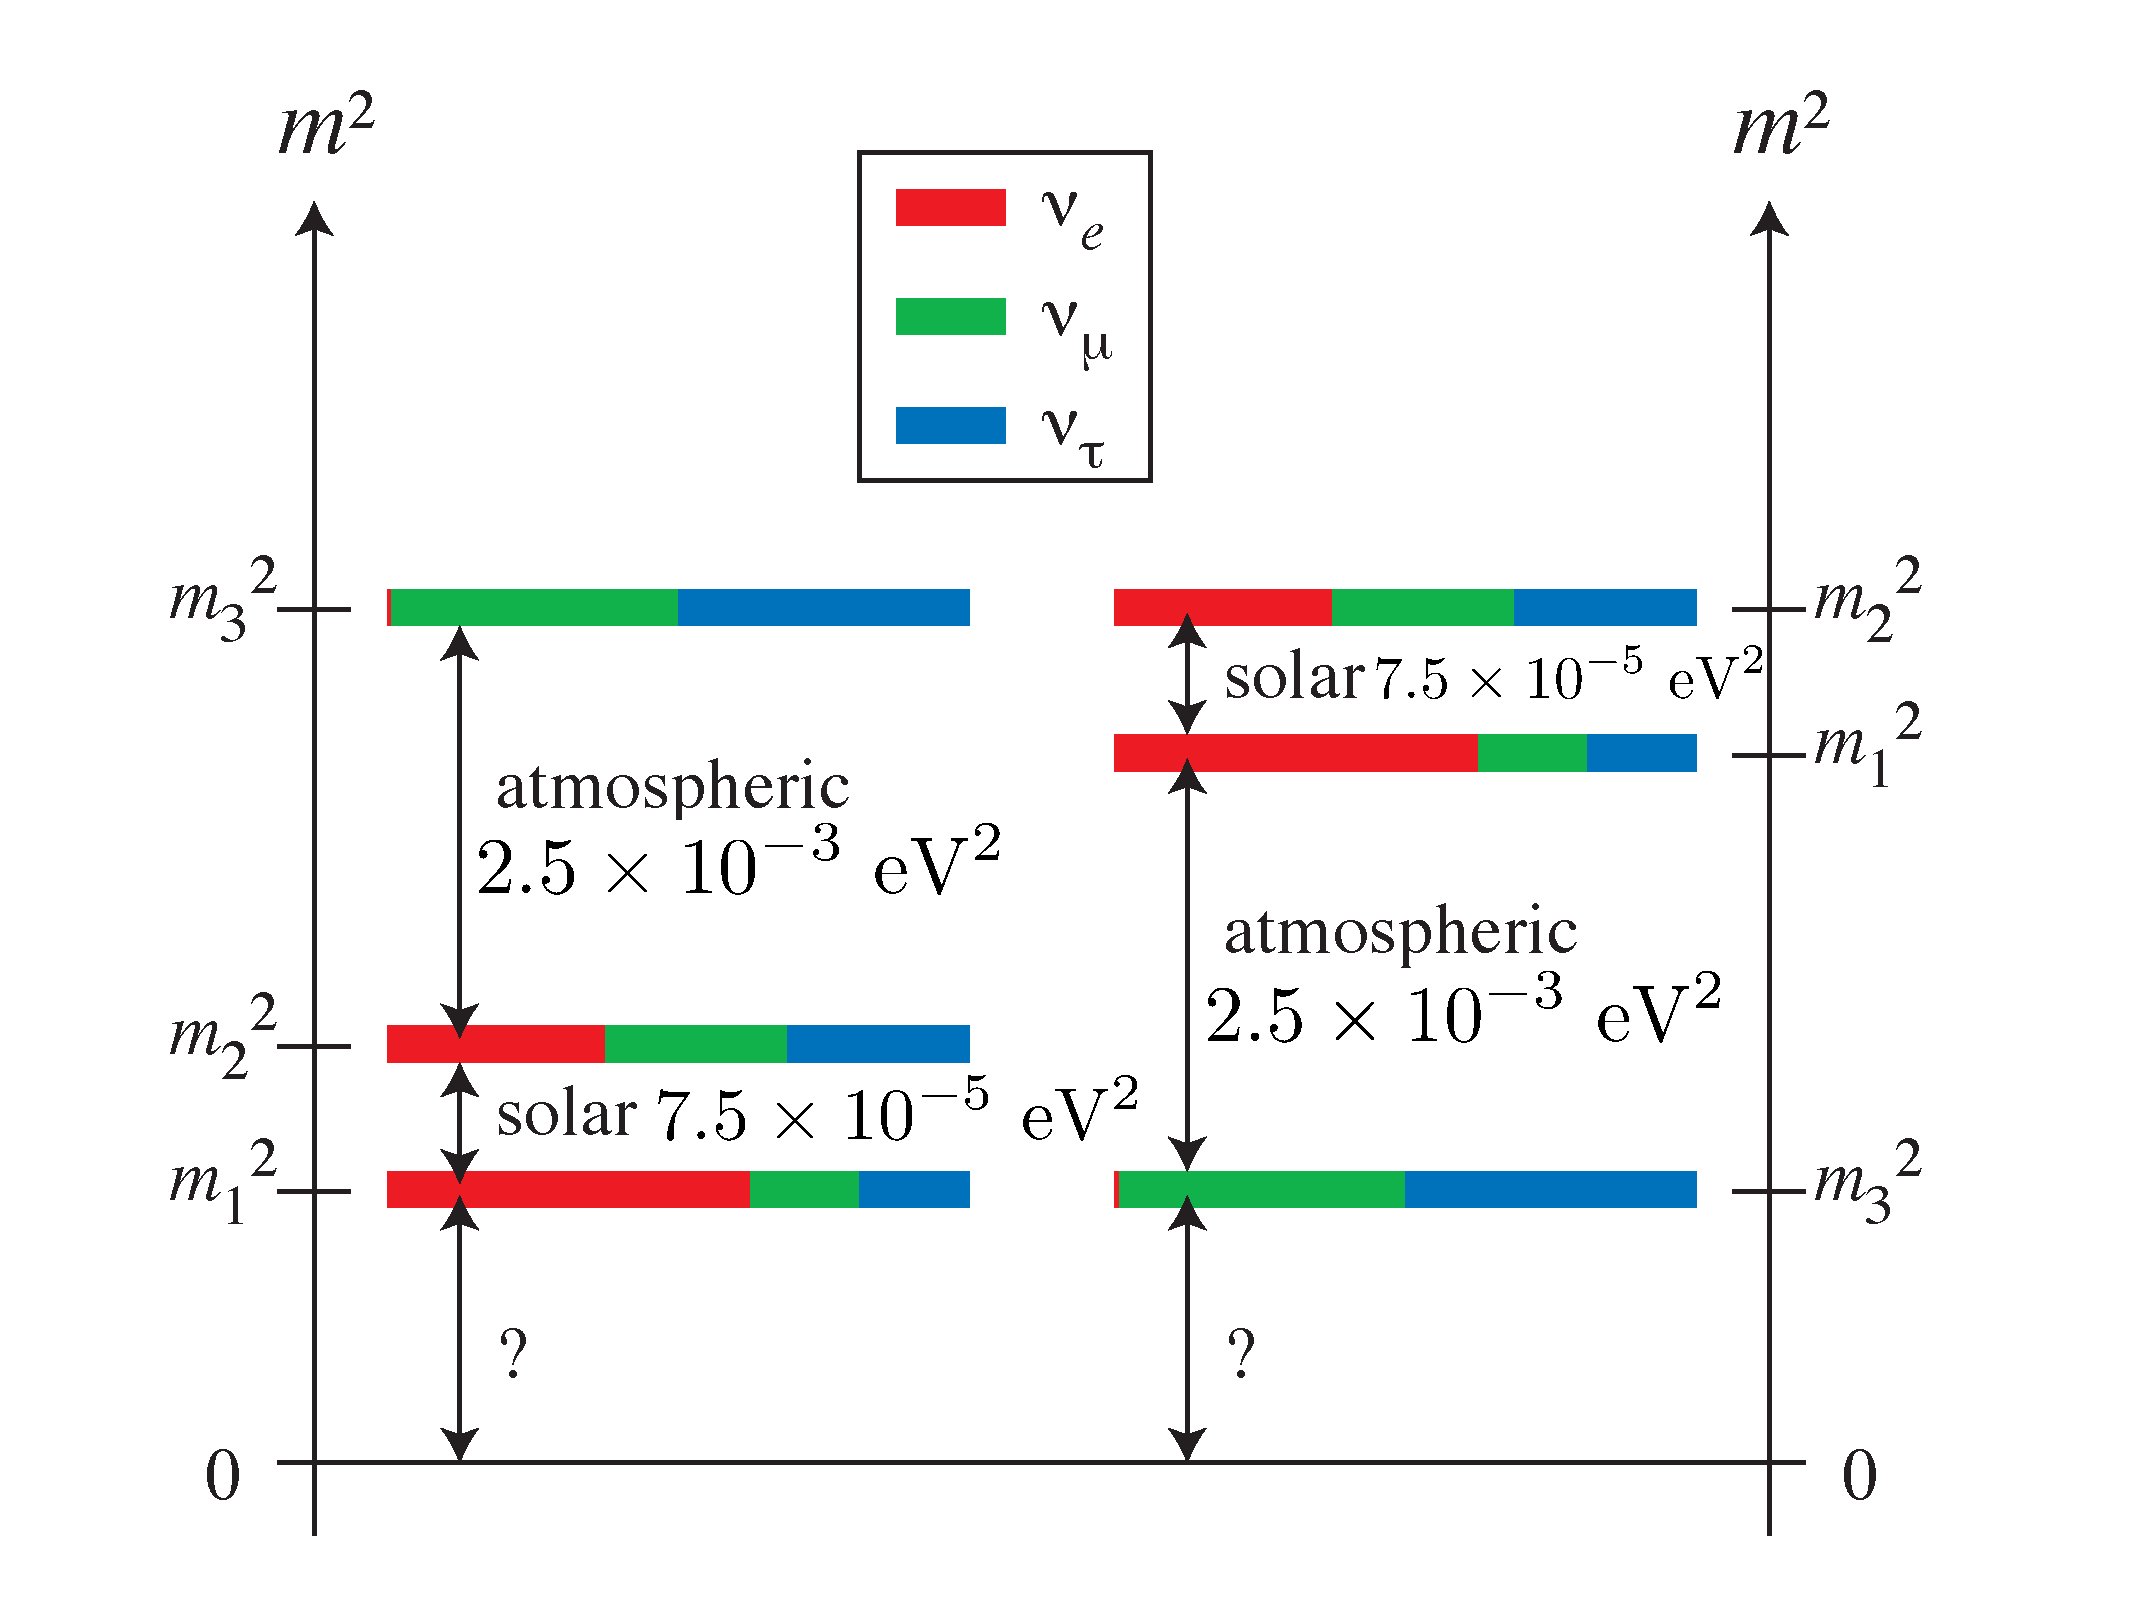
\includegraphics[width=\textwidth]{nu-detection/mass}
	\caption[Neutrino mass ordering]{%
		The two possible neutrino mass orderings arising from the unknown sign of $\dms_{31}$: normal ordering (NO) on the left and inverted ordering (IO) on the right.
		Neutrino oscillation experiments can only determine $\dms_{ij} = m_i ^ 2 - m_j ^ 2$, not the absolute mass scale.
		Also shown is the flavour content (colour bars) of the three mass eigenstates.~\cite{king}
	}
	\label{fig:nu-detection_mass}
\end{figure}

Neutrino oscillation is different in matter than in vacuum.
The neutrinos are coherently scattered off the shell electrons, similar to the propagation of light through matter.
As will be shown in Section~\ref{sec:nu-detection_interactions}, the interactions of \Pgne and \Pagne differ from the other flavours, they are possible through an additional channel.
Thus, the interaction probability of electron neutrinos is higher.
From Figure~\ref{fig:nu-detection_mass}, it can be seen, that \Pgne are primarily present in \HepParticle{\nu}{1}{} and \HepParticle{\nu}{2}{}.
Therefore, the propagation of these two is altered while \HepParticle{\nu}{3}{} is almost unaffected.
Named after its discoverers, the \gls{msw} effect~\cite{mikheyevSmirnov, wolfenstein} can be exploited to determine the mass ordering with a properly tuned $\frac{L}{E}$.


\section{\glsentryshort{dune}}
\label{sec:nu-detection_dune}
\glsreset{dune}
\glsreset{nd}
\glsreset{fd}
\glsreset{surf}
\glsreset{pot}

The \dune{}~\cite{dune1, dune2, dune3, dune4} is a long-baseline neutrino oscillation experiment measuring $P \qty(\Pgngm \rightarrow \Pgne)$ and $P \qty(\Pagngm \rightarrow \Pagne)$ planned to start data taking after 2025.
It consist of a neutrino beamline at \gls{fail} in Illinois, USA and \lartpc{} \glspl{fd} at a baseline of \SI{1300}{\kilo\metre} in the \gls{surf} in South Dakota, USA.
An artistic view of \dune{} is shown in Figure~\ref{fig:nu-detection_dune}.

\begin{figure}[htb]
	\centering
	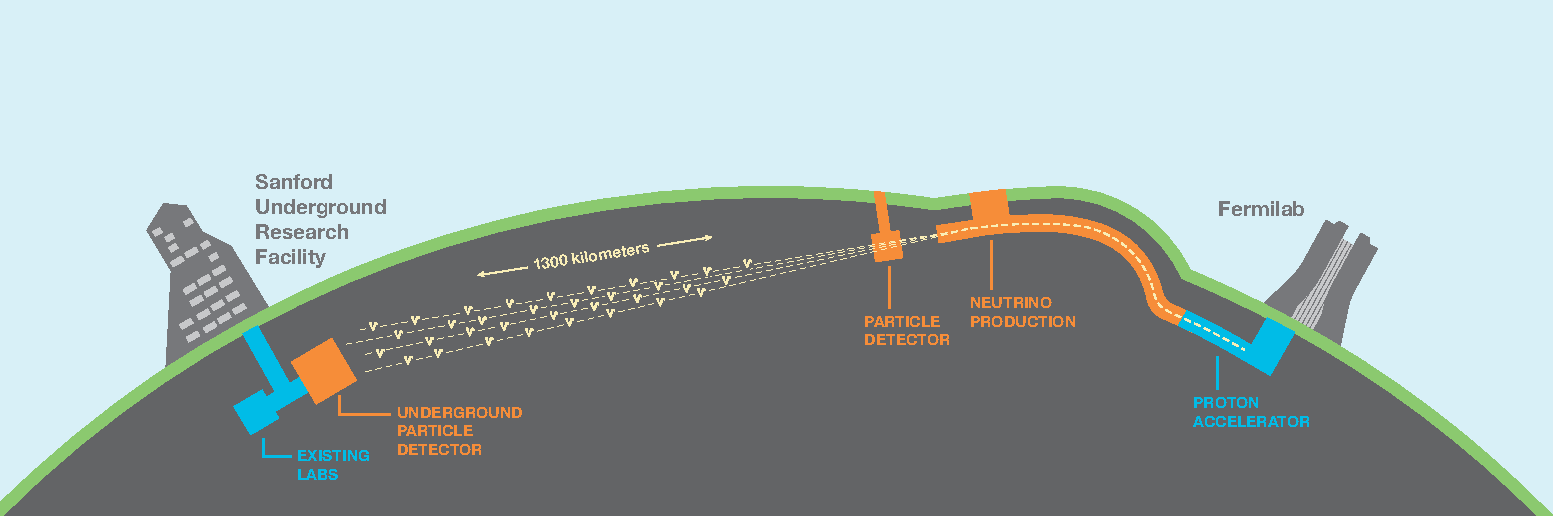
\includegraphics[width=\textwidth]{dune/dune}
	\caption[\glsentryshort{dune}]{%
		\acrshort{dune}, a next-generation long-baseline neutrino oscillation experiment consisting of a neutrino beamline and \acrshort{nd} complex at \acrshort{fail}, and \acrshort{lartpc} \acrshortpl{fd} at \acrshort{surf}.~\cite{dune1}
	}
	\label{fig:nu-detection_dune}
\end{figure}

The beamline at \gls{fail} produces pions by shooting a pulsed proton beam onto a graphite target.
A variable proton energy of \SIrange{60}{120}{\giga\electronvolt} allows for the production of different neutrino fluxes.
One pulse is called a spill and has a duration of \SI{10}{\micro\second} at a period of \SIrange{0.7}{1.2}{\second}, depending on the proton energy.
During phase one of the experiment, each spill will contain \num{7.5e13} protons resulting in an beam power of \SIrange{1.03}{1.20}{\mega\watt}.
In the later phase two, the number of protons per spill will be doubled, doubling the power as well as the average number of events per spill in the detectors.
A summary of the various proton beam configurations is given in Table~\ref{tab:nu-detection_beam-params}.
In accordance with \cite{dune2}, most calculations in this work assume the \SI{2}{\mega\watt} \SI{80}{\giga\electronvolt} beam, i.e. \num{0.2} events per tonne of argon and beam spill.
The produced pions pass through several \gls{em} focusing horns to enter a decay pipe where they decay to \Pgmp(\Pgmm) and \Pgngm(\Pagngm) according to Equation~\eqref{eq:nu-detection_pion-decay}.
By altering the polarity of the current in the focusing horns, either \Pgpp or \Pgpm can be selected primarily, enhancing the \Pgngm or \Pagngm content of the beam, respectively.
Alongside the pions, a small amount of kaons is produced as well.
These in turn can decay to \Pgne and \Pagne with a branching ratio of $\approx\SI{5}{\percent}$~\cite{pdg} producing a significant \Pgne (\Pagne) beam contamination.
The neutrino beam flux is depicted in Figure~\ref{fig:nu-detection_xsec_flux}.
Delivered neutrino flux integrated over time is usually given in \gls{pot} because the effective neutrino flux depends on several factors and can only be precisely assessed by \gls{nd} measurements.
More information on the beamline can be found in~\cite{dune2}.

\begin{table}[htb]
	\begin{minipage}{\textwidth}
		\centering
		\caption[\glsentryshort{dune} beam parameters and \glsentryshort{nd} rates]{%
			Summary of the \acrshort{dune} proton beam parameters for various configurations.
			Initially, the beamline will operate with the phase one parameters.
			Later, it will be upgraded to support the phase two parameters.
			The spill duration is \SI{10}{\micro\second} for all configurations.
			The last column gives the expected total number of neutrino interactions per tonne of argon and beam spill in the \acrshort{nd}, excluding rock events.
			It is calculated by multiplying the expected neutrino flux with the cross-section on argon from the GENIE\footnote{\url{https://genie.hepforge.org}} neutrino event generator.
			Note that these values are slightly different from the ones in Table~\ref{tab:nu-detection_beam-params} because the latter are outdated.
			In accordance with \cite{dune2}, most calculations in this work assume the \SI{2}{\mega\watt} \SI{80}{\giga\electronvolt} beam, i.e. \num{0.2} events per tonne of argon and beam spill.
			Taken from~\cite{dune3, lauraNDRates}.
		}
		\label{tab:nu-detection_beam-params}
		\begin{tabu} to \textwidth {cSSSSS}
			\toprule
			Phase &			{$E_{\Pp} \ \qty[\si{\giga\electronvolt}]$} &	{\acrshort{pot} per spill} &	{Spill period $\qty[\si{\second}]$} &	{Power $\qty[\si{\mega\watt}]$} &	{\acrshort{nd} rate $\qty[\si{evt\per\tonne_{\ce{Ar}}}]$} \\
			\midrule
			\Romannum{1} &	60 &											7.5e13 &						0.7 &									1.03 &								0.078 \\
			\Romannum{2} &	60 &											1.5e14 &						0.7 &									2.06 &								0.16 \\
			\Romannum{1} & 	80 &											7.5e13 &						0.9 &									1.07 &								0.11 \\
			\Romannum{2} &	80 &											1.5e14 &						0.9 &									2.14 &								0.21 \\
			\Romannum{1} &	120 &											7.5e13 &						1.2 &									1.20 &								0.17 \\
			\Romannum{2} &	120 &											1.5e14 &						1.2 &									2.40 &								0.33 \\
			\bottomrule
		\end{tabu}
	\end{minipage}
\end{table}

The baseline and energy spectrum of \dune{} are optimised to measure \dcp{} and determine the mass ordering.
Figure~\ref{fig:nu-detection_dune-osc} shows the (anti)neutrino oscillation probability as a function of neutrino energy at the \dune{} baseline for the normal and inverted mass ordering.
In very simple terms, \dcp{} can be derived from the difference in oscillation probability between neutrino and antineutrino mode.
The \gls{msw} effect enhances either neutrino or antineutrino oscillation depending on the mass ordering, allowing for a determination of the latter.
For more thorough sensitivity treatments, see~\cite{king, duneT2HKSens, qianVogel}.

\begin{figure}[htb]
	\centering
	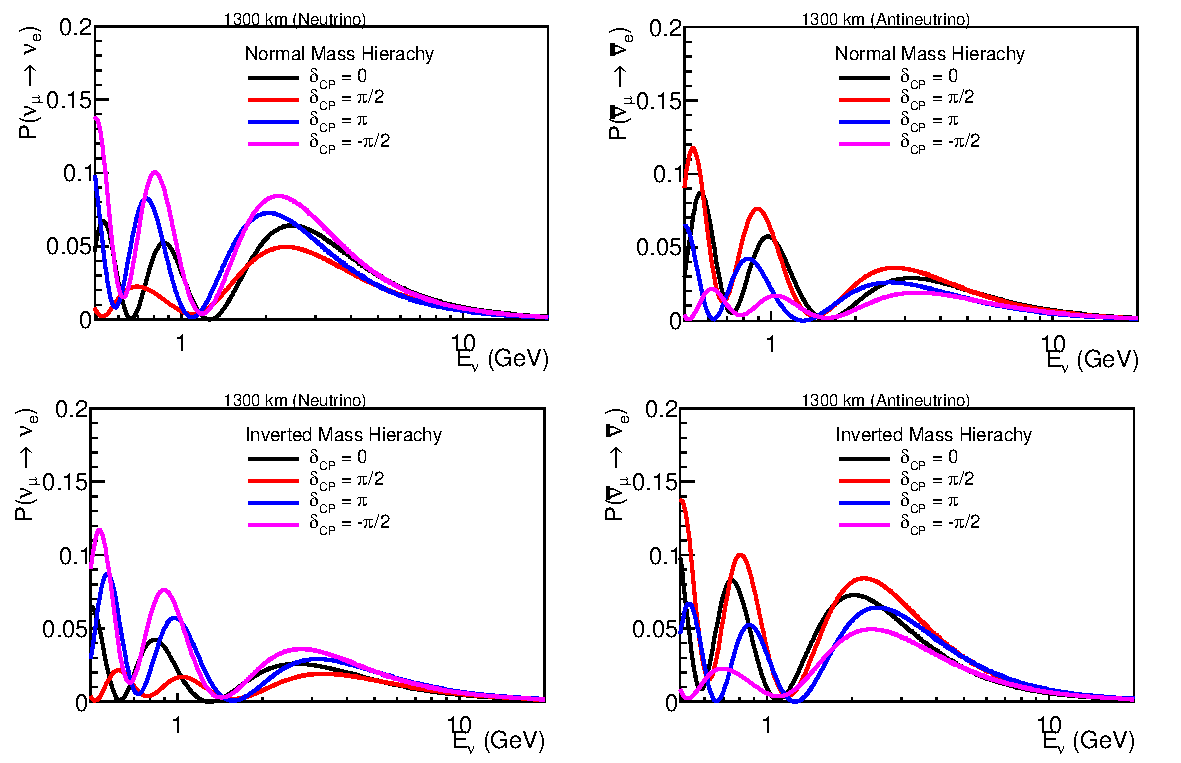
\includegraphics[width=\textwidth]{dune/LBNE_osc}
	\caption[Neutrino oscillation probabilities.]{%
		Muon to electron neutrino (left) and antineutrino (right) oscillation probability for normal (top) and inverted (bottom) mass ordering (hierarchy in the figure).
		The oscillation probabilities are calculated from equation~\eqref{eq:nu-detection_oscprob}.
		\dcp{} can be obtained from the difference between neutrino and antineutrino mode.
		The \acrshort{msw} effect either enhances the probability in neutrino or antineutrino mode depending on the mass ordering, allowing for a determination or the latter.~\cite{qianVogel}
	}
	\label{fig:nu-detection_dune-osc}
\end{figure}

Figure~\ref{fig:nu-detection_dune-sens} shows the sensitivities of \dune{} to determination of the mass ordering and discovery of \gls{cp} violation.
To reach a $3 \sigma$ sensitivity for a \SI{75}{\percent} coverage of the \dcp{} parameter space, an exposure of \SI{1320}{\kilo\tonne\mega\watt.years} is required.
Assuming the reference design of a \SI{40}{\kilo\tonne} \gls{fd} and a \SI{1}{\mega\watt} beam results in a data taking time of \SI{33}{years}.
Therefore, a beam $> \SI{1}{\mega\watt}$ is required to reach the sensitivity goal earlier.

\begin{figure}[htb]
	\centering
	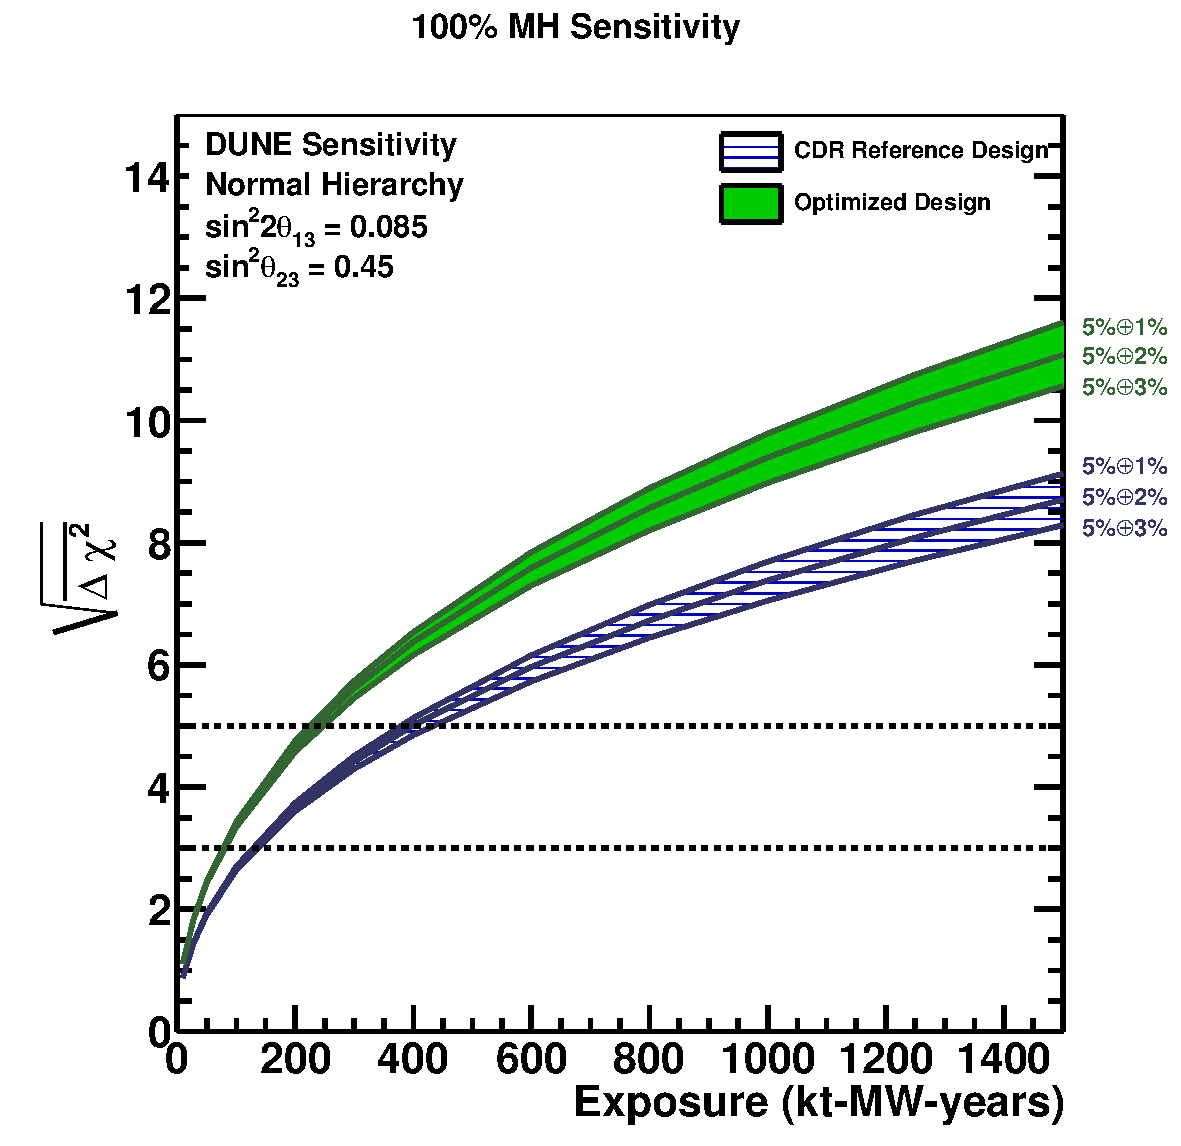
\includegraphics[width=.49\textwidth]{dune/mh_exp_syst}
	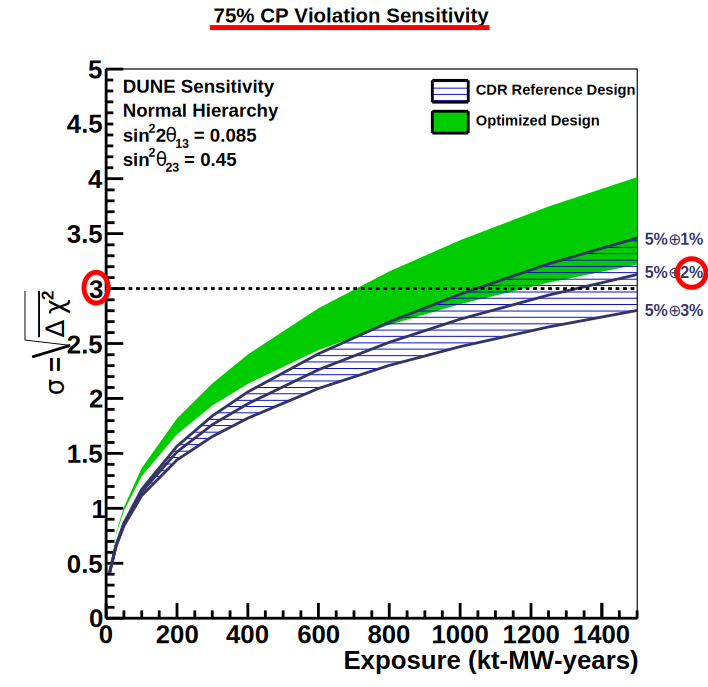
\includegraphics[width=.49\textwidth]{dune/cpv75_exp_syst}
	\caption[\glsentryshort{dune} \dcp{} sensitivity]{%
		Expected sensitivity of \acrshort{dune} to determination of the neutrino mass ordering (hierarchy, left) and discovery of \acrshort{cp} violation, i.e.\ $\dcp \neq\ 0\ \m{or}\ \pi$, (right) as a function of exposure in \si{\kilo\tonne\mega\watt.years}, assuming equal running in neutrino and antineutrino mode, for a range of values for the \Pgne and \Pagne signal normalisation uncertainties from $\SI{5}{\percent}\oplus\SI{3}{\percent}$ to $\SI{5}{\percent}\oplus\SI{1}{\percent}$.
		The sensitivities quoted are the minimum sensitivity for \SI{100}{\percent} of \dcp{} values in the case of mass ordering and \SI{75}{\percent} of \dcp{} values in the case of \acrshort{cp} violation.
		The two bands on each plot represent a range of potential beam designs described in \cite{dune2}: the blue hashed band is for the reference design and the solid green band is for the optimized design.
		For \acrshort{cp} violation sensitivities, true mass ordering is assumed to be normal but unknown.
		Taken from~\cite{dune2}.
	}
	\label{fig:nu-detection_dune-sens}
\end{figure}

Another important feature of Figure~\ref{fig:nu-detection_dune-sens} are the indicated signal normalisation uncertainties.
The aforementioned exposure assumes an uncertainty of $\SI{5}{\percent}\oplus\SI{2}{\percent}$.
In particular the second number has a significant influence on sensitivity.
A detailed explanation of this is out of the scope of this work and can be found in~\cite{dune2}.
Precise constraints of neutrino flux rate and shape by means of a \gls{nd} (in addition to hadron measurements with replica targets) are needed to reach the quoted uncertainties.
The \gls{nd} complex is placed at a distance of \SI{574}{\metre} downstream of the proton beam target.
It is important to have a \gls{nd} component employing the same target material and detector technology as the \gls{fd}, i.e.\ a \lartpc{} to eliminate the introduction of further extrapolation uncertainties.

\lartpc{}s are slow detectors, as will be explained in Chapter~\ref{chap:lartpc}.
This is problematic in the high-multiplicity \gls{nd} environment of \dune{}.
Event rates of \num{0.2} events per tonne of argon lead to significant pile-up (see Table~\ref{tab:nu-detection_beam-params}).
It is for this reason that~\cite{dune2} does not mention a \gls{nd} \lar{} component.


\section{Neutrino Interaction with Matter}
\label{sec:nu-detection_interactions}
\glsreset{cc}
\glsreset{nc}
\glsreset{qe}
\glsreset{res}
\glsreset{dis}
\glsreset{coh}
\glsreset{mec}

\begin{table}[htb]
	\centering
	\caption[\glsentryshort{dune} \glsentryshort{nd} event rates]{%
		Estimated number of interactions per tonne of argon at the \acrshort{dune} \acrshort{nd} for approximately one month (\num{1e20}~\acrshort{pot}) exposure to an (anti)neutrino beam produced from a primary proton beam of \SI{120}{\giga\electronvolt} and \SI{1.2}{\mega\watt}, taken from~\cite{dune2}.
		Note that these rates are slightly different from the ones in Table~\ref{tab:nu-detection_beam-params}.
		The reason for this is that the values below are outdated.
		However, their order of magnitude is correct and no such detailed breakdown is available for the more recent values.
		Therefore, they are presented as a rough estimate for the expected rates for the different interaction channels.
	}
	\label{tab:nu-detection_nd-rates}
	\begin{tabu} to \textwidth {llSS}
		\toprule
		Production mode &		Reaction &																														{\Pgngm beam} &		{\Pagngm beam} \\
		\midrule
		\acrshort{cc} \acrshort{qe} &			\HepProcess{\Pgngm\Pn \to \Pgmm\Pp} &																			30000 &				13000 \\
		\acrshort{nc} elastic &					\HepProcess{\Pgngm\nucleon \to \Pgngm\nucleon} & 																11000 &				6700 \\
		\acrshort{cc} \acrshort{res} &			\HepProcess{\Pgngm\Pp \to \Pgmm\Pp\Pgpp} &																		21000 &				0 \\
		\acrshort{cc} \acrshort{res} &			\HepProcess{\Pgngm\Pn \to \Pgmm\Pn\Pgpp\, (\Pp\Pgpz)} &															23000 &				0 \\
		\acrshort{cc} \acrshort{res} &			\HepProcess{\Pagngm\Pp \to \Pgmp\Pp\Pgpm\, (\Pn\Pgpz)} &														0 &					8300 \\
		\acrshort{cc} \acrshort{res} &			\HepProcess{\Pagngm\Pn \to \Pgmp\Pn\Pgpm} &																		0 &					12000 \\
		\acrshort{nc} \acrshort{res} &			\HepProcess{\Pgngm\Pp \to \Pgngm\Pp\Pgpz\, (\Pn\Pgpp)} &														7000 &				0 \\
		\acrshort{nc} \acrshort{res} &			\HepProcess{\Pgngm\Pn \to \Pgngm\Pn\Pgpp\, (\Pp\Pgpz)} &														9000 &				0 \\
		\acrshort{nc} \acrshort{res} &			\HepProcess{\Pagngm\Pp \to \Pagngm\Pp\Pgpm\, (\Pn\Pgpz)} &														0 &					3900 \\
		\acrshort{nc} \acrshort{res} &			\HepProcess{\Pagngm\Pn \to \Pagngm\Pn\Pgpm} &																	0 &					4700 \\
		\acrshort{cc} \acrshort{dis} &			\HepProcess{\Pgngm\nucleon \to \Pgmm\particles} or \HepProcess{\Pagngm\nucleon \to \Pgmp\particles} &			95000 &				24000 \\
		\acrshort{nc} \acrshort{dis} &			\HepProcess{\Pgngm\nucleon \to \Pgngm\particles} or \HepProcess{\Pagngm\nucleon \to \Pagngm\particles} &		31000 &				10000 \\
		\acrshort{cc} \acrshort{coh} \Pgpp &	\HepProcess{\Pgngm\nucleus \to \Pgmm\nucleus\Pgpp} &															930 &				0 \\
		\acrshort{cc} \acrshort{coh} \Pgpm &	\HepProcess{\Pagngm\nucleus \to \Pgmp\nucleus\Pgpm} &															0 &					800 \\
		\acrshort{nc} \acrshort{coh} \Pgpz &	\HepProcess{\Pgngm\nucleus \to \Pgngm\nucleus\Pgpz} or \HepProcess{\Pagngm\nucleus \to \Pagngm\nucleus\Pgpz} &	520 &				450 \\
		\acrshort{nc} elastic electron &		\HepProcess{\Pgngm\Pem \to \Pgngm\Pem} or \HepProcess{\Pagngm\Pem \to \Pagngm\Pem} &							16 &				11 \\
		Inverse muon decay &					\HepProcess{\Pgngm\Pem \to \Pgmm\Pgne} &																		9.5 &				0 \\
		\midrule
		Total \acrshort{cc} &			&																														170000 &			59000 \\
		Total \acrshort{cc}+\acrshort{nc} &	&																													230000 &			84000 \\
		\bottomrule
	\end{tabu}
\end{table}

Neutrinos cannot be directly detected, they need to pass on some of their energy and momentum to secondary particles that can be detected, i.e.\ they need to interact with a detection medium.
This chapter will give a brief overview of the different types of these interactions.
In general, neutrino interactions are divided into \gls{cc} and \gls{nc} mediated by charged (\PWpm) or neutral (\PZz) gauge bosons, respectively.
In a \gls{cc} interaction, the neutrino is transformed into its corresponding charged lepton while it survives an \gls{nc} interaction.
Furthermore, they can be subdivided according to the type of interaction into \gls{qe}, \gls{res}, \gls{dis}, and \gls{coh}.

\gls{qe} is characterised by the reactions
\begin{IEEEeqnarray}{C}
	\HepProcess{\Pgnl\Pn \to \Plm\Pp} \qand \HepProcess{\Pagnl\Pp \to \Plp\Pn}
\end{IEEEeqnarray}
and the kinematics are similar to that of an elastic collision, hence \gls{qe}.
Apparent from the equation above, this can only happen as a \gls{cc} interaction.

The \gls{nc} equivalent is an actual elastic interaction of a neutrino with a target nucleon according to
\begin{IEEEeqnarray}{C}
	\HepProcess{\Pgnl\nucleon \to \Pgnl\nucleon} \qq*{.}
\end{IEEEeqnarray}

\gls{res} involves the excitation of the involved nucleon to a resonant state, e.g.\
\begin{IEEEeqnarray}{C}
	\HepProcess{\Pgngm\Pp \to \Pgmm\HepParticle{\Delta}{}{++} \to \Pgmm\Pp\Pgpp}
\end{IEEEeqnarray}
where the \HepParticle{\Delta}{}{++} resonance is too short-lived to be seen by the detectors.
There are a lot of different \gls{res} interactions which all work in a similar manner.

For \gls{dis}, the momentum transfer is high enough to destroy nucleon.
The neutrino detaches a quark which in turn starts to hadronise and form jets.
The reactions are
\begin{IEEEeqnarray}{C}
	\HepProcess{\Pgnl\nucleon \to \Pl\particles} \qor \HepProcess{\Pgnl\nucleon \to \Pgnl\particles}
\end{IEEEeqnarray}
where \nucleon{} is the target nucleon and \particles{} a group of hadrons.
This reaction happens in a very similar manner to deep inelastic electron scattering off nucleons.

In a \gls{coh} reaction, the opposite happens.
The neutrino interacts with a target nucleus ($A$) as a whole but the latter is left intact as a spectator.
Instead, another particle is produced alongside the corresponding lepton. An example reaction is
\begin{IEEEeqnarray}{C}
	\HepProcess{\Pgngm\nucleus \to \Pgngm\nucleus\Pgpz}
\end{IEEEeqnarray}
where a pion is produced from a muon neutrino interacting with a target nucleus.

Inverse muon decay,
\begin{IEEEeqnarray}{C}
	\HepProcess{\Pgngm\Pem \to \Pgmm\Pgne} \qc
\end{IEEEeqnarray}
requires neutrino energies above \SI{11}{\giga\electronvolt}~\cite{dune2}, hence the low rate in Table~\ref{tab:nu-detection_nd-rates}.

Of particular importance is elastic scattering off shell electrons,
\begin{IEEEeqnarray}{C}
	\HepProcess{\Pgnl\Pem \to \Pgnl\Pem} \qor \HepProcess{\Pagnl\Pem \to \Pagnl\Pem} \qc
\end{IEEEeqnarray}
which is possible for all (anti)neutrino flavours.
For \Pgne/\Pagne, the interaction is also possible in the \gls{cc} channel via the exchange of a \PWpm boson as depicted in Figures~\ref{fig:nu-detection_nue-scat} and~\ref{fig:nu-detection_nueb-scat}.
This gives rise to a flavour-dependent term in the oscillation probability in matter, the \gls{msw} effect (see Section~\ref{sec:nu-detection_osc}).

\begin{figure}[htb]
	\centering
	\begin{fmffile}{graphics/fmf/NC-nue-scat}
		\unitlength=.4\textwidth
		\begin{fmfgraph*}(1,.5)
			\fmfpen{thin}
			\fmfstraight
			\fmfleftn{i}{2}
			\fmfrightn{o}{2}
			\fmf{fermion,label=\Pem,label.side=left}{i1,v1}
			\fmf{fermion,label=\Pem,label.side=left}{v1,o1}
			\fmf{fermion,label=\Pgnl,label.side=right}{i2,v2}
			\fmf{fermion,label=\Pgnl,label.side=right}{v2,o2}
			\fmf{boson,label=\PZz,label.side=left}{v1,v2}
			\fmfdot{v1,v2}
		\end{fmfgraph*}
	\end{fmffile}
	\begin{fmffile}{graphics/fmf/CC-nue-scat}
		\unitlength=.4\textwidth
		\begin{fmfgraph*}(1,.5)
			\fmfpen{thin}
			\fmfstraight
			\fmfleftn{i}{2}
			\fmfrightn{o}{2}
			\fmf{fermion,label=\Pem,label.side=left}{i1,v1}
			\fmf{fermion,label=\Pgne,label.side=left}{v1,o1}
			\fmf{fermion,label=\Pgne,label.side=right}{i2,v2}
			\fmf{fermion,label=\Pem,label.side=right}{v2,o2}
			\fmf{boson,label=\PWpm,label.side=left}{v1,v2}
			\fmfdot{v1,v2}
		\end{fmfgraph*}
	\end{fmffile}
	\caption[Neutrino electron scattering]{%
		\acrshort{nc} (left) and \acrshort{cc} (right) neutrino electron scattering.
	}
	\label{fig:nu-detection_nue-scat}
\end{figure}

\begin{figure}[htb]
	\centering
	\begin{fmffile}{graphics/fmf/NC-nueb-scat}
		\unitlength=.4\textwidth
		\begin{fmfgraph*}(1,.5)
			\fmfpen{thin}
			\fmfstraight
			\fmfleftn{i}{2}
			\fmfrightn{o}{2}
			\fmf{fermion,label=\Pem,label.side=left}{i1,v1}
			\fmf{fermion,label=\Pem,label.side=left}{v1,o1}
			\fmf{fermion,label=\Pagnl,label.side=right}{i2,v2}
			\fmf{fermion,label=\Pagnl,label.side=right}{v2,o2}
			\fmf{boson,label=\PZz,label.side=left}{v1,v2}
			\fmfdot{v1,v2}
		\end{fmfgraph*}
	\end{fmffile}
	\begin{fmffile}{graphics/fmf/CC-nueb-scat}
		\unitlength=.4\textwidth
		\begin{fmfgraph*}(1,.5)
			\fmfpen{thin}
			\fmfstraight
			\fmfleftn{i}{2}
			\fmfrightn{o}{2}
			\fmf{fermion,label=\Pem,label.side=left}{i1,v1}
			\fmf{fermion,label=\Pem,label.side=left}{v2,o1}
			\fmf{fermion,label=\Pagne,label.side=right}{i2,v1}
			\fmf{fermion,label=\Pagne,label.side=right}{v2,o2}
			\fmf{boson,label=\PWm,label.side=left}{v1,v2}
			\fmfdot{v1,v2}
		\end{fmfgraph*}
	\end{fmffile}
	\caption[Antineutrino electron scattering]{%
		\acrshort{nc} (left) and \acrshort{cc} (right) antineutrino electron scattering.
	}
	\label{fig:nu-detection_nueb-scat}
\end{figure}

A summary of the expected rates of the different interactions in the \dune{} \gls{nd} is given in Table~\ref{tab:nu-detection_nd-rates}.
Figure~\ref{fig:nu-detection_xsec_flux} depicts the cross-section (explained below) of neutrino interactions as a function of neutrino energy.
For comparison, the flux shapes of several experiments\footnote{The \acrfull{minerna}~\cite{minerna} is a neutrino scattering experiment at \acrshort{fail} measuring neutrino interaction cross-sections on various target materials. \acrfull{nona}~\cite{nona} is a neutrino oscillation experiment at \acrshort{fail}.} are shown (in arbitraty units).
The cross-section is split into contributions from \gls{cc} and \gls{nc} interactions.
For \gls{cc}, the individual contributions from \gls{res} and 1p1h+2p2h are shown, where $x$p$y$h refers to $x$ particles and $y$ holes; i.e.\ the target nucleus is missing $y$ nucleons after the interactions.
1p1h corresponds to a \gls{cc} \gls{qe} interaction whereas in 2p2h interactions a virtual meson is exchanged inside the target nucleus, also called \gls{mec}.
Interactions involving \glspl{mec} are important because they can mimic the detector response of \gls{cc} \gls{qe} events.

\begin{figure}[htb]
	\centering
	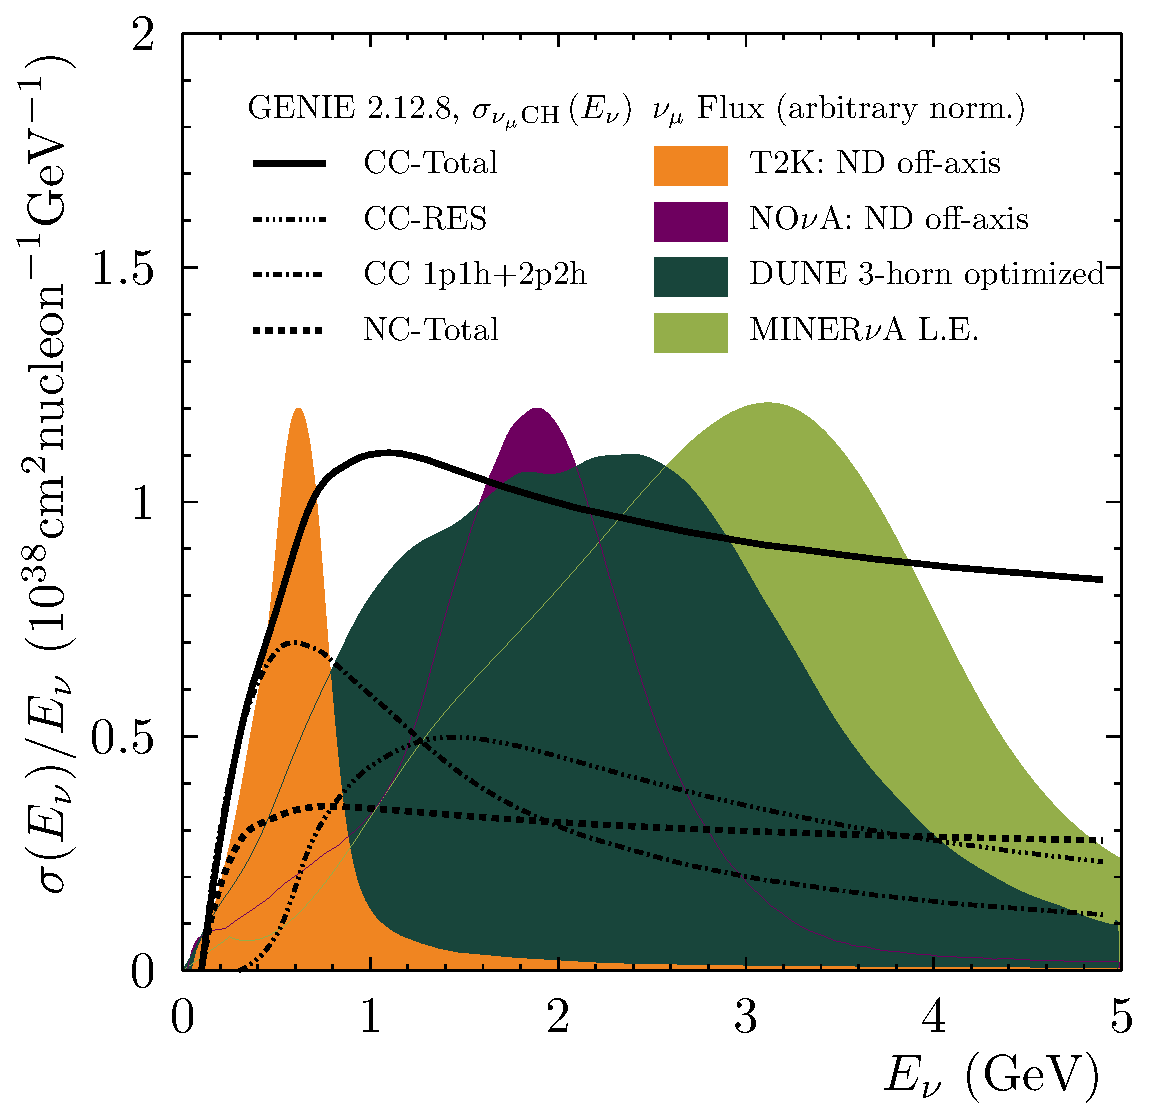
\includegraphics[width=\textwidth]{nu-detection/flux_and_xsec_from_luke}
	\caption[Neutrino interaction cross-section and beam fluxes]{%
		Neutrino interaction cross-section per nucleon as a function of neutrino energy in \si{\giga\electronvolt}.
		The cross-section is split into contributions from \acrshort{cc} and \acrshort{nc} interactions.
		For \acrshort{cc}, the individual contribution from \acrshort{res} interactions is shown, as well as from the sum of 1p1h and 2p2h.
		The latter two correspond to the \acrshort{qe} channel and interactions involving \acrshortpl{mec}, respectively.
		Overlaid are the flux shapes of various beam experiments in arbitrary units.
		The \acrshort{dune} flux is drawn for the optimised beam design with an \SI{80}{\giga\electronvolt} proton beam operating in neutrino mode.
		Kindly provided by L.\ Pickering and C.\ Wilkinson~\cite{xsec_luke} with \acrshort{dune} flux information from L.\ Fields~\cite{lauraNDRates}.
	}
	\label{fig:nu-detection_xsec_flux}
\end{figure}

To better understand the meaning of Figure~\ref{fig:nu-detection_xsec_flux}, a brief explanation of the cross-section concept is given here.
For a beam consisting of particles \particlea{} incident on a target made of particles \particleb{}, the rate of the interaction \HepProcess{\particlea\particleb \to \particles} is given by
\begin{IEEEeqnarray}{rCl}
	R_{\particles} & = & \phi_{\particlea} N_{\particleb} \sigma_{\particlea\particleb\particles} \qc
\end{IEEEeqnarray}
where $\phi_{\particlea}$ is the flux of beam particles, $N_{\particleb}$ is the number of target particles, and $\sigma_{\particlea\particleb\particles}$ is the cross-section.
Therefore, the cross-section
\begin{IEEEeqnarray}{rCl}
	\sigma_{\particlea\particleb\particles} & = & \frac{R_X}{\phi_{\particlea} N_{\particleb}}
\end{IEEEeqnarray}
is a measure for the interaction rate $R_{\particles}$ normalised by the number of both, beam and target, particles.
As flux is given in units of inverse time and area, and interaction rate in inverse time, the cross-section needs to have the dimension of an area.


\section{Final State Detection}
\label{sec:nu-detection_fs}

In order to be able to detect particles, they need to interact with a detection medium.
This section will describe the most important interaction of charged particles as well as neutral particles with matter.
It is focused on charged interactions as these are the most important ones for \lartpc{}s.
As a measure of the interaction strength, the energy loss per distance or stopping power $\dv{E}{x}$ is used.
Where not otherwise mentioned, this section is based on~\cite{grupen}.

The main interaction of charged particles with matter happens on atomic electrons.
That is why for most of these interactions, one needs to treat the interaction of electrons separately.
For all other charged particles, the stopping power is described by the Bethe-Bloch formula
\begin{IEEEeqnarray}{rCl}
	- \frac{1}{\rho} \dv{E}{x} & = &
	4 \pi N_{\m{A}} r_{\Pe} ^ 2 m_{\Pe} c ^ 2 z ^ 2 \frac{Z}{A} \frac{1}{\beta ^ 2}
	\qty[\ln(\frac{2 m_{\Pe} c ^ 2 \gamma ^ 2 \beta ^ 2}{I}) - \beta ^ 2 - \frac{\delta}{2}] \qc
	\label{eq:nu-detection_bethe-bloch}
\end{IEEEeqnarray}
where
\begin{description}
	\item[$\rho$] is the density of the absorber material,
	\item[$N_{\m{A}}$] is Avogadro's number,
	\item[$r_{\Pe} = \frac{1}{4 \pi \varepsilon_{\m{0}}} \frac{\si{\elementarycharge} ^ 2}{m_{\Pe} c ^ 2}$] is the classical electron radius using the permittivity of free space $\varepsilon_{\m{0}}$,
	\item[$m_{\Pe}$] is the electron mass,
	\item[$z$] is the charge of the incident particle,
	\item[$Z$] is the atomic number of the absorber,
	\item[$A$] is the atomic weight of the absorber,
	\item[$\beta = \frac{v}{c}$] with $v$ the velocity of the incident particle,
	\item[$\gamma = \frac{E}{m_0 c ^ 2}$] with $E$ the energy and $m_0$ the rest mass of the incident particle,
	\item[$I$] is the mean excitation energy of the absorber material which can be approximated by
		\begin{IEEEeqnarray}{rCl}
			I & = & 16 Z ^ {0.9} \si{\electronvolt} \quad \m{for} \quad Z > 1 \qc
		\end{IEEEeqnarray}
	\item[$\delta$] is a parameter describing the screening of the extended transverse electric field of relativistic incident particles by the charge density of the atomic electrons of the absorber.
\end{description}
Equation~\eqref{eq:nu-detection_bethe-bloch} describes the stopping power of particles with $m_0 \gg m_{\Pe}$ by ionisation and excitation of the atoms in the absorber material.
As the stopping power is proportional to the electron density and thus to the mass density of the absorber material, it is often divided by the latter.
Thus, Equation~\eqref{eq:nu-detection_bethe-bloch} actually gives the so called mass stopping power.
The only remaining dependence on the absorber material is $\frac{Z}{A}$ which is $\approx 0.5$ for most light materials, and the mean excitation energy which only contributes logarithmically.

\begin{figure}[htb]
	\centering
	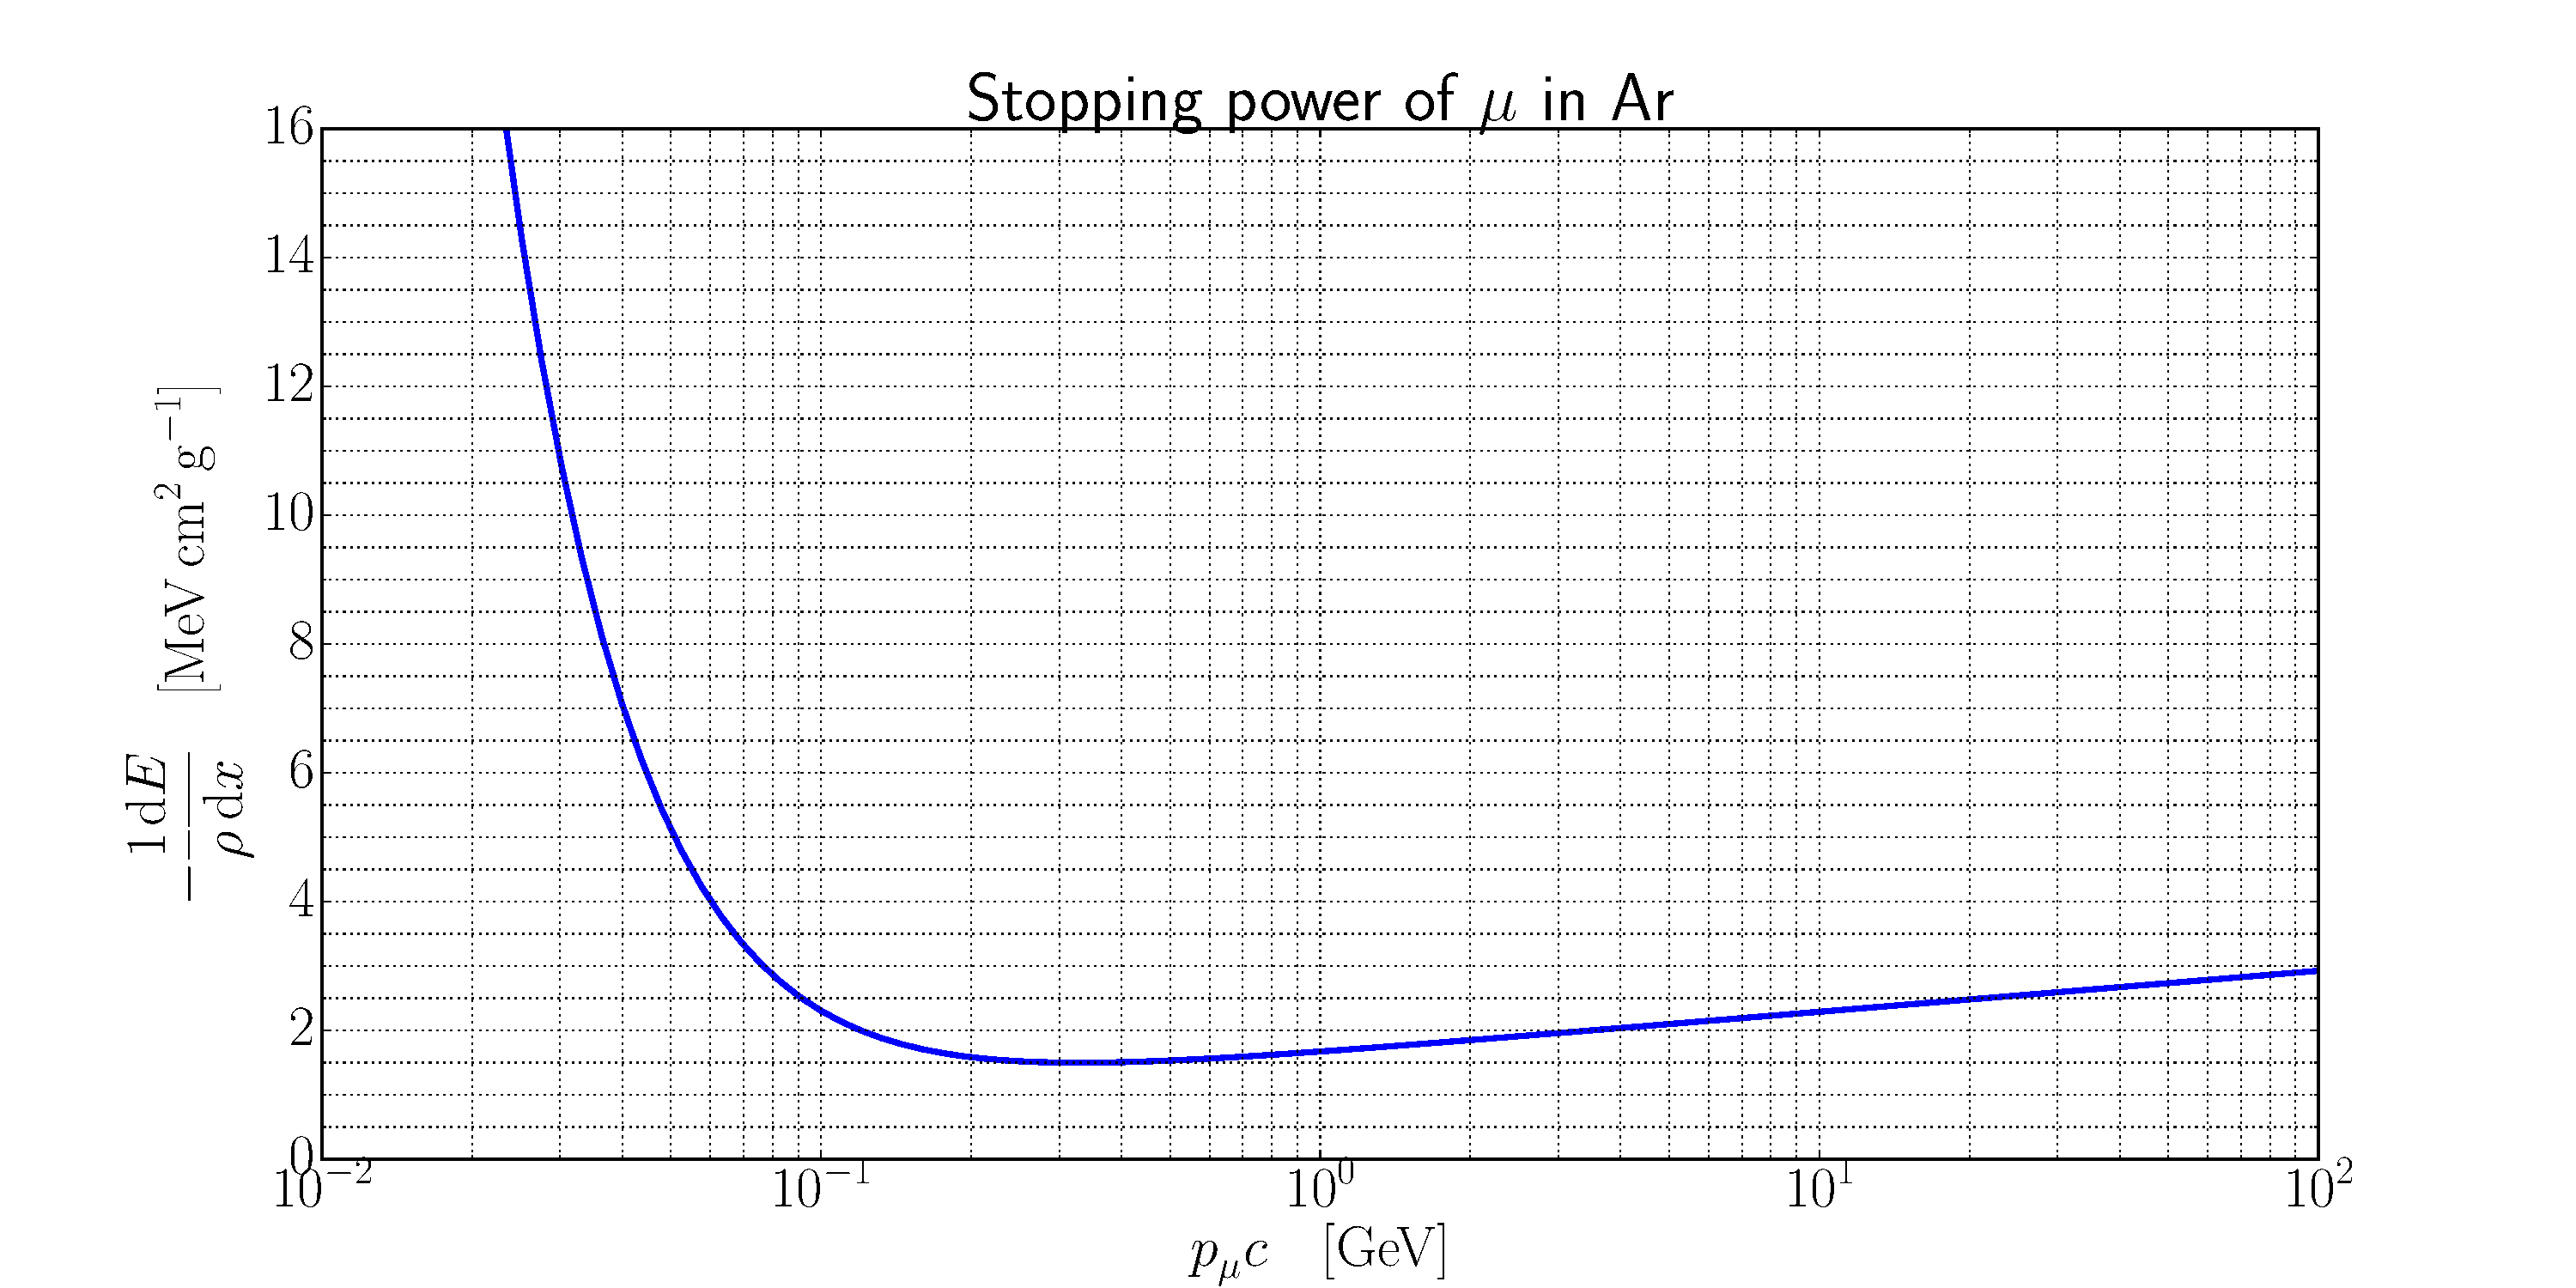
\includegraphics[width=\textwidth]{nu-detection/bethe_bloch}
	\caption[Stopping power]{%
		Bethe-Bloch stopping power of \Pgm in \ce{Ar}.
	}
	\label{fig:nu-detection_bethe-bloch}
\end{figure}

Figure~\ref{fig:nu-detection_bethe-bloch} shows the mass stopping power of muons in argon neglecting the $\frac{\delta}{2}$ term for simplicity.
As can be seen, there is a broad minimum which is characteristic of the Bethe-Bloch formula.
Particles in this momentum range are called \glspl{mip}.
They are important for detectors because this energy loss is a measure for the required energy resolution of a detector.
As mentioned, the mass stopping power only loosely depends on the absorber material and therefore, its minimum is
\begin{IEEEeqnarray}{rCl}
	\eval{- \frac{1}{\rho} \dv{E}{x}}_{\m{min}} & \approx & \SI{2}{\mega\electronvolt\centi\meter\squared\per\gram}
\end{IEEEeqnarray}
for singly charged incident particles on most (light) absorbers.
To the left of the minimum, the stopping power rises with a strong $\frac{1}{\beta ^ 2}$ dependence.
A consequence of this is a pronounced peak in the energy loss as a function of the travelled distance of a particle near its stopping point.
This \emph{Bragg peak} is especially important for radiation therapy with heavy charged particles (e.g.\ protons).
After the minimum, the stopping power rises again with a logarithmic dependence on $\beta$ and the mean excitation energy of the absorber $I$.
The reason for this so called \emph{logarithmic rise} is the extension of the transverse electric field of the incident particle in the relativistic regime.
Due to increasing shielding of the transverse electric field by the shell electrons of the absorber materials, taken into account by the $\frac{\delta}{2}$ term, the rise is only asymptotic.
For electrons and positrons, Equation~\eqref{eq:nu-detection_bethe-bloch} does not hold because their mass is equal to the mass of the atomic electrons of the absorber.
The stopping power changes further for electrons because the incident particle cannot be distinguished form its collision partner.
On the other hand, a positron will be annihilated upon stop by an electron which needs to be taken into account as well.
The equivalent of Equation~\eqref{eq:nu-detection_bethe-bloch} for \Pepm can be found in~\cite{grupen}.

At high velocities further effects come into play.
\emph{Bremsstrahlung} describes the radiation energy loss of a fast charged particle in the Coulomb field of the absorber nuclei.
It can be described by
\begin{IEEEeqnarray}{rCl}
	- \frac{1}{\rho}\dv{E}{x} & = & \frac{E}{X_{\m{0}}}
	\label{eq:nu-detection_bremsstrahlung}
\end{IEEEeqnarray}
where
\begin{IEEEeqnarray}{rCl}
	X_{\m{0}} & = & \frac{A}{4 \alpha N_A Z \qty(Z + 1) \qty(\frac{1}{4 \pi \varepsilon_{\m{0}}} \frac{\si{\elementarycharge} ^ 2}{m c ^ 2}) ^ 2 \ln(183 Z ^ {- \frac{1}{3}})}
	\label{eq:nu-detection_radiationlength}
\end{IEEEeqnarray}
is the \emph{radiation length} of the absorber material using
\begin{description}
	\item[$\alpha$] $\approx \frac{1}{137}$ the fine-structure constant and
	\item[$m$] the mass of the incident particle.
\end{description}
Again, the energy loss is proportional to the density of the absorber and for convenience, divided by the latter.
Bremsstrahlung is emitted in interactions of the incident particle with the absorber nuclei ($\propto Z ^ 2$) as well as with the atomic electrons of the absorber ($\propto Z$).
By neglecting the latter, one obtains the important relation
\begin{IEEEeqnarray}{rCl}
	X_{\m{0}} ^ {- 1} & \propto & Z ^ 2
\end{IEEEeqnarray}
as opposed to the $\propto Z$ dependence of the Bethe-Bloch formula.
Equation~\eqref{eq:nu-detection_bremsstrahlung} also holds for electrons as long as $E \gg \frac{m_{\Pe} c ^ 2}{\alpha Z ^ {\frac{1}{3}}}$.
Furthermore, looking at the dependence on the mass of the incident particle, one finds
\begin{IEEEeqnarray}{rCl}
	X_{\m{0}} & \propto & m ^ 2
\end{IEEEeqnarray}
using Equation~\eqref{eq:nu-detection_radiationlength}.
Therefore, the radiation length of an absorber material is usually given for electrons and the relation
\begin{IEEEeqnarray}{rCl}
	X_{\m{0}} & = & X_{\m{0}}^{\Pe} \frac{m ^ 2}{m_{\Pe} ^ 2}
\end{IEEEeqnarray}
can be used to get the radiation length for any charged particle of mass $m$.
Radiation losses play a significant role only at energies much higher than the energy of \glspl{mip}.
Using Equations~\eqref{eq:nu-detection_bethe-bloch} and~\eqref{eq:nu-detection_bremsstrahlung}, one can define a \emph{critical energy} $E_{\m{c}}$ by
\begin{IEEEeqnarray}{rCl}
	\eval{\dv{E}{x}_{\m{ion}}}_{E_{\m{c}}} & = & \eval{\dv{E}{x}_{\m{brems}}}_{E_{\m{c}}}
	\label{eq:nu-detection_ec}
\end{IEEEeqnarray}
at which radiation losses take over from ionisation losses.
Similar to the radiation length, the critical energy is proportional to $m ^ 2$.
Thus, it is most important for electrons while for other particles it becomes significant only at very high energies.
If we take an iron absorber for instance, we get $E_c^{\Pe} = \SI{20.7}{\mega\electronvolt}$ and $E_c^{\Pgm} = \SI{890}{\giga\electronvolt}$.

At high energies, there are additional types of radiation loss taking place, for example direct electron-pair production and photonuclear interactions.
They shall not be described here.
Instead, only their $\propto E$ relation similar to bremsstrahlung losses shall be mentioned.
A description of those effects can be found in~\cite{grupen}.

In addition to the processes described above, charged particles traversing matter also undergo scattering in the Coulomb field of the nuclei of the traversed medium.
Accordingly, this process is called \emph{\gls{mcs}}.
The \gls{rms} of the \emph{scattering-angle distribution}
\begin{IEEEeqnarray}{rCl}
	\Theta_{\m{\glsentryshort{rms}}} & = & \frac{\SI{13.6}{\mega\electronvolt}}{\beta c p} z \sqrt{\frac{2 x}{X_{\m{0}}}} \qty[1 + 0.038 \ln(\frac{x}{X_{\m{0}}})]
	\label{eq:nu-detection_highland}
\end{IEEEeqnarray}
is defined by the momentum $p$, velocity $\beta c$ and charge $z$ of the scattered particle, and the thickness of the scattering medium $\frac{x}{X_{\m{0}}}$ in radiation lengths.
The distinct momentum dependence of this so-called \emph{Highland formula} can be used to reconstruct the momentum of the incident particle provided the angular resolution of the detector is fine enough.

Concerning the interactions of charged particles with matter, there is one important note regarding detectors:
While charge produced in interactions (i.e.\ ionisation) can be detected directly, light (i.e.\ excitation photons and photon radiation) first needs to be converted to charge to be detected.

The three most important interactions converting photons to charge are the \emph{photoelectric effect}, \emph{Compton Scattering}, and \emph{pair production}.
All of them have in common that they attenuate photon beams exponentially according to
\begin{IEEEeqnarray}{rCl}
	I & = & I_0 e ^ {- \mu x}
\end{IEEEeqnarray}
where $I_0$ and $I$ is the intensity before and after passing the absorber, respectively.
The thickness of the absorber is given by $x$ and
\begin{IEEEeqnarray}{rCl}
	\mu & = & \frac{N_A}{A} \sum_i \sigma_i
	\label{eq:nu-detection_mass-att-coeff}
\end{IEEEeqnarray}
is the \emph{mass attenuation coefficient} defined by the sum of the cross-sections $\sigma_i$ of the different interaction processes.

At low energies (ionisation energy $\le E_{\Pgg} \le \SI{100}{\kilo\electronvolt}$), photons primarily undergo conversion to charge by the photoelectric effect.
The photon is absorbed by an atom of the absorber which in turn is ionised and thus ejects one of its shell electrons.
The cross-section is given by
\begin{IEEEeqnarray}{rCl}
	\sigma_{\m{photo}} & = & \qty(\frac{32}{\epsilon ^ 7}) ^ \frac{1}{2} \alpha ^ 4 Z ^ 5 \sigma_{\m{Th}}^{\Pe} \qc
\end{IEEEeqnarray}
where
\begin{description}
	\item[$\epsilon = \frac{E_{\Pgg}}{m_{\Pe} c ^ 2}$] is the reduced photon energy and
	\item[$\sigma_{\m{Th}}^{\Pe} = \frac{8}{3} \pi r_{\Pe} ^ 2 = \SI{6.65e-25}{\centi\meter\squared}$] is the \emph{Thomson cross-section} for elastic scattering of photons on electrons.
\end{description}

For energies $\approx \SI{1}{\mega\electronvolt}$, Compton scattering dominates the interaction of photons with matter.
Thereby, the photon is not absorbed by the atom but simply scatters off one of its shell electrons with the cross-section
\begin{IEEEeqnarray}{rCl}
	\sigma_{\m{c}} & = & 2 \pi r_{\Pe} ^ 2 Z \left\{\qty[\frac{1 + \epsilon}{\epsilon ^ 2}] \qty[\frac{2 \qty(1 + \epsilon)}{1 + 2 \epsilon} - \frac{1}{\epsilon} \ln(1 + 2 \epsilon)]\right.\\
	& & \left. + \frac{1}{2 \epsilon} \ln(1 + 2 \epsilon) - \frac{1 + 3 \epsilon}{\qty(1 + 2 \epsilon) ^ 2}\right\} \qc
\end{IEEEeqnarray}
obtained from the Klein-Nishina formula.
As only part of the photon's energy is absorbed while the rest is scattered, it makes sense to divide this cross-section into a scattering cross-section
\begin{IEEEeqnarray}{rCl}
	\sigma_{\m{cs}} & = & \frac{E_{\Pgg}'}{E_{\Pgg}}
\end{IEEEeqnarray}
and an absorption cross-section
\begin{IEEEeqnarray}{rCl}
	\sigma_{\m{ca}} & = & \sigma_{\m{c}} - \sigma_{\m{cs}} \qc
	\label{eq:nu-detection_sigma-compton}
\end{IEEEeqnarray}
where $E_{\Pgg}$ and $E_{\Pgg}'$ is the energy of the photon before and after scattering, respectively.

At $E_{\Pgg} \ge 2 m_{\Pe} c ^ 2$, photons are capable of producing pairs of \Pep\Pem.
Because of momentum conservation, this process can only happen in the Coulomb field of a so called spectator particle.
As pair-production in the field of an electron is strongly suppressed, the spectator is usually a nucleus of the absorber material.
Therefore, the cross-section of pair-production depends on the shielding of the Coulomb field by the shell electrons and thus on the proximity to the nucleus.
Eventually, this results in an energy dependence.
The cross-section is given by
\begin{IEEEeqnarray}{rCl}
	\sigma_{\m{pair}} & = & 4 \alpha r_{\Pe} ^ 2 Z ^ 2 \qty(\frac{7}{9} \ln 2 \epsilon - \frac{109}{54})
\end{IEEEeqnarray}
for $1 \ll \epsilon < \frac{1}{\alpha Z ^ {\frac{1}{3}}}$, and
\begin{IEEEeqnarray}{rCl}
	\sigma_{\m{pair}} & = & 4 \alpha r_{\Pe} ^ 2 Z ^ 2 \qty[\frac{7}{9} \ln(\frac{183}{Z ^ {\frac{1}{3}}}) - \frac{1}{54}]
\end{IEEEeqnarray}
for $\epsilon \gg \frac{1}{\alpha Z ^ {\frac{1}{3}}}$.

As mentioned above, for Compton scattering, two different cross-sections are defined, $\sigma_{\m{cs}}$ for the scattered energy and $\sigma_{\m{ca}}$ for the absorbed energy.
Consequentially, there are also different definitions of the coefficient $\mu$ in Equation~\eqref{eq:nu-detection_mass-att-coeff}.
Replacing the total Compton cross-section $\sigma_{\m{c}}$ by $\sigma_{\m{ca}}$ from Equation~\eqref{eq:nu-detection_sigma-compton}, one gets the \emph{mass absorption coefficient} $\mu_{\m{a}}$, only taking into account photon absorption processes.
While $\mu$ is more precisely called the \emph{total mass attenuation coefficient}.

An interesting effect takes place for \Pepm traversing material at energies higher than the critical energy $E_{\m{c}}$ defined by Equation~\eqref{eq:nu-detection_ec}.
In this regime, the energy loss is dominated by bremsstrahlung for \Pepm and by pair production for photons.
This leads to an \emph{\gls{em} cascade} or \emph{shower} where \Pepm and \Pgg produce each other alternately in a self-sustaining process.
The mean free path of a photon before pair production
\begin{IEEEeqnarray}{rCl}
	\lambda_{\m{prod}} & = & \frac{9}{7}X_{\m{0}}
\end{IEEEeqnarray}
is very close to the mean free path of an \Pepm before bremsstrahlung, the radiation length $X_{\m{0}}$.
Therefore, the number of particles participating in the shower doubles roughly every radiation length resulting in an exponential growth.
This allows \gls{em} showers to be approximated by the following rather simple model.
When the average energy per paticle drops below the critical energy, ionisation losses begin to dominate over radiative losses for \Pepm and Compton and photoelectric effect over pair production for photons.
At this point, the shower reaches its maximum and
\begin{IEEEeqnarray}{rCl}
	t_{\m{max}}^{\m{EM}} & = & \frac{\ln(\frac{E}{E_{\m{c}}})}{\ln(2)}
\end{IEEEeqnarray}
is its longitudinal extent in radiation lengths.
The \emph{Molière radius}
\begin{IEEEeqnarray}{rCl}
	R_{\m{M}}^{\m{EM}} & = & \frac{\SI{21}{\mega\electronvolt}}{E_{\m{c}}} X_{\m{0}}
\end{IEEEeqnarray}
is the transversal extent of the shower divided by the the material density.
Both $t_{\m{max}}^{\m{EM}}$ and $R_{\m{M}}^{\m{EM}}$ are important benchmarks for the dimensioning of \gls{em} calorimeters.
Naturally, a photon in the energy range where pair production dominates will produce a shower as well.
On the other hand, \Pgmpm can also start \gls{em} cascades, if their energy is high enough to produce bremsstrahlung.

Similarly, hadrons interacting with matter via the strong force can produce cascades as well.
As opposed to the \gls{em} showers governed only by \Pepm and \Pgg, the hadronic process is much more complex because many different secondary particle can be involved.
Hadrons start to shower because they mainly interact inelastically with matter, producing secondary strongly interacting particles.
That is why the hadronic cross-section
\begin{IEEEeqnarray}{rCl}
	\sigma_{\m{total}} & = & \sigma_{\m{elastic}} + \sigma_{\m{inel}}
\end{IEEEeqnarray}
is usually split.
From $\sigma_{\m{inel}}$, one can derive the \emph{interaction length}
\begin{IEEEeqnarray}{rCl}
	\lambda_{\m{int}} & = & \frac{A}{N_{\m{A}} \rho \sigma_{\m{inel}}}
\end{IEEEeqnarray}
which describes the absorption of hadrons in matter according to
\begin{IEEEeqnarray}{rCl}
	N & = & N_{\m{0}} e ^ {- \frac{x}{\lambda_{\m{int}}}}
\end{IEEEeqnarray}
with the initial number of hadrons $N_{\m{0}}$ and number of hadrons $N$ after a distance $x$ of absorber material.
For absorbers with $Z \geq 6$, the interaction length is much larger than the radiation length $X_{\m{0}}$ meaning that hadronic calorimeters usually need to be much larger than their \gls{em} counterparts.
Experimental data shows that hadronic showers from a few \si{\giga\electronvolt} to a few \SI{100}{\giga\electronvolt} can be approximated by similar parameters as \gls{em} showers.
The shower maximum is reached at
\begin{IEEEeqnarray}{rCl}
	t_{\m{max}}^{\m{had}} & = & 0.2 \ln(\frac{E}{\si{\giga\electronvolt}}) + 0.7
\end{IEEEeqnarray}
interaction lengths.
From this, the longitudinal extent containing \SI{95}{\percent} is given by
\begin{IEEEeqnarray}{rCl}
	L_{0.95}^{\m{had}} & = & t_{\m{max}}^{\m{had}} + 2.5 \qty(\frac{E}{\si{\giga\electronvolt}}) ^ {0.13} \qc
	\label{eq:nu-detection_hardon-long}
\end{IEEEeqnarray}
in interaction lengths again.
Transversally, \SI{95}{\percent} of the shower are contained within a cylinder of radius
\begin{IEEEeqnarray}{rCl}
	R_{0.95}^{\m{had}} & \leq & \lambda_{\m{int}}
	\label{eq:nu-detection_hardon-trans}
\end{IEEEeqnarray}
which is independent of the energy and smaller for high-Z materials~\cite{hardon}.